\documentclass[11pt,a4paper]{article}

\usepackage[utf8]{inputenc}
\usepackage[T1]{fontenc}
\usepackage[italian]{babel}
\usepackage[margin=2.5cm]{geometry}
\usepackage{float}
\usepackage{graphicx}
\usepackage{subcaption}
\usepackage{amsmath}
\usepackage{amssymb}
\usepackage{siunitx}
\usepackage[hidelinks]{hyperref}

\usepackage{pgfplots}
\pgfplotsset{compat=1.18}
\usetikzlibrary{positioning,arrows.meta,calc,fit,backgrounds}
\definecolor{matlabblue}{rgb}{0.000,0.447,0.741}
\definecolor{matlaborange}{rgb}{0.850,0.325,0.098}

\usepackage[acronym, shortcuts]{glossaries}
\newacronym{rir}{RIR}{Room Impulse Response}
\newacronym{sfc}{SFC}{Sound Field Control}
\newacronym{imsaf}{IMSAF}{Improved Multiband-Structured Subband Adaptive Filter}
\newacronym{mimo}{MIMO}{Multiple-Input Multiple-Output}
\newacronym{siso}{SISO}{Single-Input Single-Output}
\newacronym{nlms}{NLMS}{Normalized Least Mean Square}
\newacronym{nm}{NM}{Normalized Misalignment}
\newacronym{lfe}{LFE}{Low Frequency Effects}

\title{IMSAF based RIR tracking}
\author{Michele Sulis \and Mauro Michele Maria Costantino}
\date{\today}


%% Indice documento

%% Introduzione
%%
%% Algortimo
%%		Descrizione algoritmo
%% 		Schema a blocchi (riadattato dal paper, senza sfc)
%%		Richiamo banco DFT (teoria)
%%
%% Simulazioni (MATLAB)
%%  	SISO 
%% 			(introduzione)
%% 			Confronto filtri (plot in frequenza)
%% 			Confronto risultati
%% 				NM
%%				RIR Tempo
%% 				RIR Frequenza
%% 		MIMO
%% 			(introduzione)
%% 			Ingressi scorrelati (-60 dB)
%%			MIMO con correlazione realistica (-9dB)
%%			Ruolo della decorrelazione intra-canale (P) - analisi con rumore colorato
%%			Segnali stereo e test vari
%%
%% Implementazione (C/C++)
%%		Schema NUTS
%%		Impostazione codice (snippet o semplicemente struttura)
%%			plugin.cpp
%%			ecc..
%%		Risultati (più RIR Tutte le prove varie)
%%			Grafici H
%%
%% Risultati finali e futuri sviluppi

\begin{document}
	
	\maketitle
	
	\section{Introduzione}
	
	Questo documento raccoglie, in forma cronologica, lo sviluppo e la sperimentazione di un algoritmo di stima e tracciamento della risposta impulsiva della stanza, o \ac{rir}, basato su filtraggio adattativo in sottobande, nel contesto dei sistemi di \ac{sfc} \cite{11249060, 11464373}.
	
	L'algoritmo di riferimento appartiene alla famiglia \ac{imsaf}: il segnale di eccitazione e i segnali captati dai microfoni vengono scomposti in sottobande tramite un \emph{banco filtri DFT}e, in ciascuna sottobanda, un filtro adattativo di tipo \ac{nlms} stima la porzione corrispondente della RIR.
	La struttura in sottobande appiattisce lo spettro visto da ciascun filtro adattativo, riducendo la correlazione del segnale in ingresso e accelerando la convergenza rispetto a un adattamento a banda piena.
	
	Il lavoro è organizzato seguendo l'ordine cronologico delle implementazioni realizzate. 
	Si parte da una configurazione \ac{siso} (un altoparlante, un microfono) per validare il banco filtri e la ricostruzione della RIR, confrontando diverse scelte di filtro prototipo.
	Si estende poi al caso \ac{mimo} (più altoparlanti, più microfoni), affrontando il problema dell'\emph{identificabilità} dovuto alla correlazione tra i canali di eccitazione e le tecniche di decorrelazione necessarie a una stima accurata.
	
	Infine, l'algoritmo validato in simulazione viene implementato in C++ come plugin per la piattaforma real-time NU-Tech \cite{nutech}.
	Il passaggio dall'elaborazione offline di MATLAB a quella a frame in tempo reale richiede una riorganizzazione dell'algoritmo: gestione della continuità tra frame consecutivi tramite buffer di overlap e indici temporali globali, buffer circolari per gli stati dei filtri, e stima ricorsiva delle grandezze che in simulazione erano calcolate sull'intero segnale.

	\section{IMSAF based RIR tracking}
	L'obiettivo di questo lavoro è implementare un algoritmo di tracciamento della \ac{rir} ispirato a \cite{11464373}, scorporandolo dall'applicazione \ac{sfc} in cui è presentato in letteratura.
	Nell'articolo originale, infatti, il tracciamento è asservito a un sistema di controllo del campo acustico che si alterna alla stima dei percorsi \cite{11249060}; qui si isola il solo blocco di identificazione, poiché la \ac{rir} ricostruita costituisce un'informazione utile a valle per algoritmi più vari: \ac{sfc}, controllo attivo del rumore, cancellazione d'eco acustica, equalizzazione di stanza.
	
	La struttura implementata è rappresentata schematicamente in Figura \ref{fig:mimo_diagram}, riadattata da \cite{11464373} omettendo la parte \ac{sfc}.
	Il flusso è il seguente: il vettore dei segnali sorgente $\mathbf{x}(n)\in\mathbb{R}^{L}$ ($L$ canali, con $n$ indice temporale a banda piena) viene decomposto in $I$ sottobande e decimato di un fattore $D$ (Sez. \ref{ssec:dft_bank}), ottenendo i segnali di sottobanda $\mathbf{x}_i(k) \in\mathbb{C}^L$ (con $i=1,\dots,I$ indice di sottobanda e $k$ indice temporale nel dominio decimato); questi vengono decorrelati tramite modulazione di fase (Sez. \ref{ssec:ph_mod}) e risintetizzati nel vettore $\mathbf{s}(n)\in\mathbb{R}^{L}$ dei segnali fisicamente inviati agli altoparlanti.
	La stanza, descritta dalla matrice $\mathbf{H}(n)\in\mathbb{R}^{M\times LK}$ delle \ac{rir} vere (dove $K$ è la lunghezza della \ac{rir} e $n$ ne indica l'eventuale tempovarianza), restituisce ai microfoni i segnali $\mathbf{y}(n)\in\mathbb{R}^{M}$ ($M$ microfoni); il modello ingresso uscita in sottobanda è formalizzato nella Sez. \ref{ssec:model_ident} (Eq. \ref{eq:subband_model}).
	Sia i segnali degli altoparlanti sia quelli dei microfoni vengono nuovamente analizzati in sottobande e, in ciascuna sottobanda, una matrice di filtri adattativi $\hat{\mathbf{H}}_i(k)\in\mathbb{C}^{M\times LK_i}$ ne stima la porzione corrispondente. Poiché l'identificazione avviene interamente in sottobanda, il filtro non modella la \ac{rir} originale ma la sua versione filtrata dal banco di analisi e allungata dalla convoluzione con il prototipo di lunghezza $V$ (Sez.~\ref{ssec:dft_bank}); la lunghezza della \ac{rir} in sottobanda è quindi $K_i=\lceil (K+V-1)/D\rceil$.
	L'adattamento è guidato dall'errore di predizione (Sez. \ref{ssec:filter_update}), mentre il segnale in sottobanda, sbiancato da uno stadio di predizione lineare (Sez. \ref{ssec:whitening}), fornisce la direzione dell'aggiornamento; il passo è pesato in modo inversamente proporzionale alla potenza media di ciascuna sottobanda (Sez. \ref{ssec:weights}).
	Al termine, le \ac{rir} a banda piena vengono ricostruite dalle stime in sottobanda (Sez.~\ref{ssec:h_recon}) e confrontate con quelle vere tramite \ac{nm} (Sez. \ref{ssec:nm_metric}).

	\begin{figure}[H]
		\centering
		% Schema a blocchi del sistema MIMO implementato.
% Richiede nel preambolo: \usetikzlibrary{positioning,arrows.meta,calc,fit,backgrounds}
% Da includere con: % Schema a blocchi del sistema MIMO implementato.
% Richiede nel preambolo: \usetikzlibrary{positioning,arrows.meta,calc,fit,backgrounds}
% Da includere con: % Schema a blocchi del sistema MIMO implementato.
% Richiede nel preambolo: \usetikzlibrary{positioning,arrows.meta,calc,fit,backgrounds}
% Da includere con: \input{figures/mimo_diagram}
\begin{tikzpicture}[
    font=\footnotesize,
    >={Stealth[length=2.2mm]},
    blk/.style={draw, thick, rounded corners=2pt, fill=white, align=center,
                minimum height=10mm, inner sep=2.2mm},
    room/.style={blk, fill=orange!12, draw=orange!60!black},
    sum/.style={draw, thick, circle, fill=white, inner sep=0pt, minimum size=4.2mm},
    sig/.style={->, thick},
    note/.style={font=\scriptsize, text=black!60, align=center},
    grouplab/.style={font=\scriptsize\bfseries, text=black!70},
    busN/.style={font=\scriptsize, inner sep=1pt},
  ]

  % ============ Decorrelazione (catena orizzontale in alto) ============
  \node[blk] (ana1) at (1.0,0) {Banco di analisi\\DFT ($I$, $\downarrow D$)};
  \node[blk] (pmod) at (5.35,0) {Modulazione\\di fase\\[-1pt] {\scriptsize\color{black!60} $e^{\mathrm{j}\alpha_i \sin(2\pi f_l k D / f_s)}$}};
  \node[blk] (syn1) at (9.6,0) {Banco di sintesi\\DFT ($I$, $\uparrow D$)};

  \draw[sig] (-2.0,0) -- node[above, pos=0.25]{$\mathbf{x}(n)$} (ana1);
  \draw[thick] ($(-2.0,0)!0.3!(ana1.west)+(-2pt,-4pt)$) -- +(4pt,8pt)
        node[busN, below=3mm]{$L$};
  \draw[sig] (ana1) -- node[above]{$\mathbf{x}_i(k)$} (pmod);
  \draw[sig] (pmod) -- node[above]{$\mathbf{s}_i(k)$} (syn1);

  % ============ Verso stanza e ri-analisi ============
  \coordinate (tap) at (12.4,-2.4);
  \node[room] (roomH) at (12.4,-4.4) {Stanza \\$\mathbf{H}(n)$};
  \node[blk] (ana2) at (2.6,-4.4) {Banco di analisi\\DFT ($I$, $\downarrow D$)};
  \node[blk] (ana3) at (6.6,-4.4) {Banco di analisi\\DFT ($I$, $\downarrow D$)};

  \draw[sig] (syn1.east) -- (12.4,0) -- (roomH.north);
  \node[right] at (12.5,-1.0) {$\mathbf{s}(n)$};
  \draw[thick] ($(12.4,-1.55)+(-4pt,-2pt)$) -- +(8pt,4pt)
        node[busN, right=2.5mm]{$L$};
  \fill (tap) circle (1.3pt);
  \draw[sig] (tap) -- (2.6,-2.4) -- (ana2.north);
  \draw[sig] (roomH.west) -- node[above]{$\mathbf{y}(n)$} (ana3.east);
  \draw[thick] ($(roomH.west)!0.5!(ana3.east)+(-2pt,-4pt)$) -- +(4pt,8pt)
        node[busN, below=3mm]{$M$};

  % ============ Nucleo IMSAF ============
  \coordinate (sdot) at (2.6,-5.9);
  \node[blk] (pred) at (1.0,-7.1) {Predizione\\lineare\\[-1pt]{\scriptsize\color{black!60} $\underline{\mathbf{u}}_i = \underline{\mathbf{s}}_i - \mathbf{S}_i \mathbf{a}_i$}\\[-2pt] {\scriptsize\color{black!60} ordine $P$}};
  \node[blk] (wei)  at (4.6,-7.1) {Pesi di sottobanda\\[-1pt] {\scriptsize\color{black!60} $w_i \propto 1/\sigma_i$}};
  \node[sum] (esum) at (6.6,-9.2) {};

  \draw[sig] (ana2) -- node[right, pos=0.35]{$\mathbf{s}_{i}(k)$} (sdot) -- (2.6,-8.6);
  \fill (sdot) circle (1.3pt);
  \draw[sig] (sdot) -| (pred.north);
  \draw[sig] (sdot) -| (wei.north);
  \draw[sig] (pred.south) -- node[left, pos=0.5]{$\underline{\mathbf{u}}_i(k)$} (1.0,-8.6);
  \draw[sig] (wei.south) -- node[right, pos=0.5]{$w_i$} (4.6,-8.6);

  \draw[sig] (ana3) -- node[right, pos=0.55]{$\mathbf{y}_{i}(k)$} (esum);
  \node[busN] at ($(esum.north east)+(0.26,0.1)$) {$+$};
  \node[busN] at ($(esum.west)+(-0.3,-0.26)$) {$-$};

  % Retroazione dell'errore: dal ramo orizzontale sale in verticale e
  % attraversa in obliquo il blocco dei filtri (disegnato dopo, quindi
  % in primo piano): la freccia entra dal basso e riesce dall'alto.
  \draw[sig] (esum.south) -- node[right, pos=0.4]{$\mathbf{e}_{i}(k)$} (6.6,-10.3)
        -- (0.7,-10.3) -- (0.7,-10) -- (2.3,-8.25);

  \node[blk, minimum width=53mm] (hhat) at (2.6,-9.2) {Filtri adattativi\\di sottobanda $\hat{\mathbf{H}}_i(k)$};
  \draw[sig] (hhat.east) -- node[above]{$\hat{\mathbf{y}}_{i}(k)$} (esum);

  % ============ Ricostruzione e confronto (riga in basso) ============
  \node[blk] (rec) at (2.6,-13.3) {Ricostruzione fullband\\[-1pt] {\scriptsize\color{black!60} impulso $\to$ analisi $\to \hat{\mathbf{H}}_i \to$ sintesi}};
  \node[blk] (nm)  at (9,-13.3) {Calcolo NM\\[-1pt] {\scriptsize\color{black!60} confronto con $\mathbf{H}(n)$}};
  \draw[sig] (hhat.south) -- node[right, pos=0.68]{$\hat{\mathbf{H}}(k)$}
        (rec.north);
  \draw[thick] ($(hhat.south)!0.88!(rec.north)+(-4pt,-1.5pt)$) -- +(8pt,5pt)
        node[busN, right=2.5mm]{$M \times LK_{i} \times I$};
  \draw[sig] (rec.east) -- node[above]{$\hat{\mathbf{H}}(n)$} (nm.west);
  \draw[thick] ($(rec.east)!0.5!(nm.west)+(-2pt,-4pt)$) -- +(4pt,8pt)
        node[busN, below=3mm]{$M \times LK$};

  % ============ Gruppi con etichette in basso a destra ============
  \coordinate (fitExcS) at (11.1,-1.35);
  \coordinate (fitTrkS) at (8.2,-10.85);
  \coordinate (fitTrkN) at (0,0 |- ana2.north);
  \coordinate (fitTrkN) at ([yshift=4mm]ana2.north);
  
  \begin{scope}[on background layer]
    \node[fill=gray!12, rounded corners=4pt, fit=(ana1)(pmod)(syn1)(fitExcS),
          inner sep=4mm] (gExc) {};
    \node[grouplab, anchor=south east, align=right] at ($(gExc.south east)+(-0.18,0.1)$)
          {Decorrelazione dei segnali di eccitazione\\ [-1pt]{\tiny per ogni sottobanda ($i = 1,\dots,I$)}};
    \coordinate (fitTrkW) at ([xshift=4mm]gExc.west |- ana2.center);
    \node[fill=cyan!8, rounded corners=4pt,
    fit=(ana2)(ana3)(hhat)(esum)(pred)(wei)(fitTrkS)(fitTrkW)(fitTrkN),
    inner sep=4mm] (gTrk) {};
    \node[grouplab, anchor=south east, align=right] at ($(gTrk.south east)+(-0.18,0.1)$)
          {Tracciamento IMSAF\\ [-1pt]{\tiny per ogni sottobanda ($i = 1,\dots,I$)}};
  \end{scope}

\end{tikzpicture}

\begin{tikzpicture}[
    font=\footnotesize,
    >={Stealth[length=2.2mm]},
    blk/.style={draw, thick, rounded corners=2pt, fill=white, align=center,
                minimum height=10mm, inner sep=2.2mm},
    room/.style={blk, fill=orange!12, draw=orange!60!black},
    sum/.style={draw, thick, circle, fill=white, inner sep=0pt, minimum size=4.2mm},
    sig/.style={->, thick},
    note/.style={font=\scriptsize, text=black!60, align=center},
    grouplab/.style={font=\scriptsize\bfseries, text=black!70},
    busN/.style={font=\scriptsize, inner sep=1pt},
  ]

  % ============ Decorrelazione (catena orizzontale in alto) ============
  \node[blk] (ana1) at (1.0,0) {Banco di analisi\\DFT ($I$, $\downarrow D$)};
  \node[blk] (pmod) at (5.35,0) {Modulazione\\di fase\\[-1pt] {\scriptsize\color{black!60} $e^{\mathrm{j}\alpha_i \sin(2\pi f_l k D / f_s)}$}};
  \node[blk] (syn1) at (9.6,0) {Banco di sintesi\\DFT ($I$, $\uparrow D$)};

  \draw[sig] (-2.0,0) -- node[above, pos=0.25]{$\mathbf{x}(n)$} (ana1);
  \draw[thick] ($(-2.0,0)!0.3!(ana1.west)+(-2pt,-4pt)$) -- +(4pt,8pt)
        node[busN, below=3mm]{$L$};
  \draw[sig] (ana1) -- node[above]{$\mathbf{x}_i(k)$} (pmod);
  \draw[sig] (pmod) -- node[above]{$\mathbf{s}_i(k)$} (syn1);

  % ============ Verso stanza e ri-analisi ============
  \coordinate (tap) at (12.4,-2.4);
  \node[room] (roomH) at (12.4,-4.4) {Stanza \\$\mathbf{H}(n)$};
  \node[blk] (ana2) at (2.6,-4.4) {Banco di analisi\\DFT ($I$, $\downarrow D$)};
  \node[blk] (ana3) at (6.6,-4.4) {Banco di analisi\\DFT ($I$, $\downarrow D$)};

  \draw[sig] (syn1.east) -- (12.4,0) -- (roomH.north);
  \node[right] at (12.5,-1.0) {$\mathbf{s}(n)$};
  \draw[thick] ($(12.4,-1.55)+(-4pt,-2pt)$) -- +(8pt,4pt)
        node[busN, right=2.5mm]{$L$};
  \fill (tap) circle (1.3pt);
  \draw[sig] (tap) -- (2.6,-2.4) -- (ana2.north);
  \draw[sig] (roomH.west) -- node[above]{$\mathbf{y}(n)$} (ana3.east);
  \draw[thick] ($(roomH.west)!0.5!(ana3.east)+(-2pt,-4pt)$) -- +(4pt,8pt)
        node[busN, below=3mm]{$M$};

  % ============ Nucleo IMSAF ============
  \coordinate (sdot) at (2.6,-5.9);
  \node[blk] (pred) at (1.0,-7.1) {Predizione\\lineare\\[-1pt]{\scriptsize\color{black!60} $\underline{\mathbf{u}}_i = \underline{\mathbf{s}}_i - \mathbf{S}_i \mathbf{a}_i$}\\[-2pt] {\scriptsize\color{black!60} ordine $P$}};
  \node[blk] (wei)  at (4.6,-7.1) {Pesi di sottobanda\\[-1pt] {\scriptsize\color{black!60} $w_i \propto 1/\sigma_i$}};
  \node[sum] (esum) at (6.6,-9.2) {};

  \draw[sig] (ana2) -- node[right, pos=0.35]{$\mathbf{s}_{i}(k)$} (sdot) -- (2.6,-8.6);
  \fill (sdot) circle (1.3pt);
  \draw[sig] (sdot) -| (pred.north);
  \draw[sig] (sdot) -| (wei.north);
  \draw[sig] (pred.south) -- node[left, pos=0.5]{$\underline{\mathbf{u}}_i(k)$} (1.0,-8.6);
  \draw[sig] (wei.south) -- node[right, pos=0.5]{$w_i$} (4.6,-8.6);

  \draw[sig] (ana3) -- node[right, pos=0.55]{$\mathbf{y}_{i}(k)$} (esum);
  \node[busN] at ($(esum.north east)+(0.26,0.1)$) {$+$};
  \node[busN] at ($(esum.west)+(-0.3,-0.26)$) {$-$};

  % Retroazione dell'errore: dal ramo orizzontale sale in verticale e
  % attraversa in obliquo il blocco dei filtri (disegnato dopo, quindi
  % in primo piano): la freccia entra dal basso e riesce dall'alto.
  \draw[sig] (esum.south) -- node[right, pos=0.4]{$\mathbf{e}_{i}(k)$} (6.6,-10.3)
        -- (0.7,-10.3) -- (0.7,-10) -- (2.3,-8.25);

  \node[blk, minimum width=53mm] (hhat) at (2.6,-9.2) {Filtri adattativi\\di sottobanda $\hat{\mathbf{H}}_i(k)$};
  \draw[sig] (hhat.east) -- node[above]{$\hat{\mathbf{y}}_{i}(k)$} (esum);

  % ============ Ricostruzione e confronto (riga in basso) ============
  \node[blk] (rec) at (2.6,-13.3) {Ricostruzione fullband\\[-1pt] {\scriptsize\color{black!60} impulso $\to$ analisi $\to \hat{\mathbf{H}}_i \to$ sintesi}};
  \node[blk] (nm)  at (9,-13.3) {Calcolo NM\\[-1pt] {\scriptsize\color{black!60} confronto con $\mathbf{H}(n)$}};
  \draw[sig] (hhat.south) -- node[right, pos=0.68]{$\hat{\mathbf{H}}(k)$}
        (rec.north);
  \draw[thick] ($(hhat.south)!0.88!(rec.north)+(-4pt,-1.5pt)$) -- +(8pt,5pt)
        node[busN, right=2.5mm]{$M \times LK_{i} \times I$};
  \draw[sig] (rec.east) -- node[above]{$\hat{\mathbf{H}}(n)$} (nm.west);
  \draw[thick] ($(rec.east)!0.5!(nm.west)+(-2pt,-4pt)$) -- +(4pt,8pt)
        node[busN, below=3mm]{$M \times LK$};

  % ============ Gruppi con etichette in basso a destra ============
  \coordinate (fitExcS) at (11.1,-1.35);
  \coordinate (fitTrkS) at (8.2,-10.85);
  \coordinate (fitTrkN) at (0,0 |- ana2.north);
  \coordinate (fitTrkN) at ([yshift=4mm]ana2.north);
  
  \begin{scope}[on background layer]
    \node[fill=gray!12, rounded corners=4pt, fit=(ana1)(pmod)(syn1)(fitExcS),
          inner sep=4mm] (gExc) {};
    \node[grouplab, anchor=south east, align=right] at ($(gExc.south east)+(-0.18,0.1)$)
          {Decorrelazione dei segnali di eccitazione\\ [-1pt]{\tiny per ogni sottobanda ($i = 1,\dots,I$)}};
    \coordinate (fitTrkW) at ([xshift=4mm]gExc.west |- ana2.center);
    \node[fill=cyan!8, rounded corners=4pt,
    fit=(ana2)(ana3)(hhat)(esum)(pred)(wei)(fitTrkS)(fitTrkW)(fitTrkN),
    inner sep=4mm] (gTrk) {};
    \node[grouplab, anchor=south east, align=right] at ($(gTrk.south east)+(-0.18,0.1)$)
          {Tracciamento IMSAF\\ [-1pt]{\tiny per ogni sottobanda ($i = 1,\dots,I$)}};
  \end{scope}

\end{tikzpicture}

\begin{tikzpicture}[
    font=\footnotesize,
    >={Stealth[length=2.2mm]},
    blk/.style={draw, thick, rounded corners=2pt, fill=white, align=center,
                minimum height=10mm, inner sep=2.2mm},
    room/.style={blk, fill=orange!12, draw=orange!60!black},
    sum/.style={draw, thick, circle, fill=white, inner sep=0pt, minimum size=4.2mm},
    sig/.style={->, thick},
    note/.style={font=\scriptsize, text=black!60, align=center},
    grouplab/.style={font=\scriptsize\bfseries, text=black!70},
    busN/.style={font=\scriptsize, inner sep=1pt},
  ]

  % ============ Decorrelazione (catena orizzontale in alto) ============
  \node[blk] (ana1) at (1.0,0) {Banco di analisi\\DFT ($I$, $\downarrow D$)};
  \node[blk] (pmod) at (5.35,0) {Modulazione\\di fase\\[-1pt] {\scriptsize\color{black!60} $e^{\mathrm{j}\alpha_i \sin(2\pi f_l k D / f_s)}$}};
  \node[blk] (syn1) at (9.6,0) {Banco di sintesi\\DFT ($I$, $\uparrow D$)};

  \draw[sig] (-2.0,0) -- node[above, pos=0.25]{$\mathbf{x}(n)$} (ana1);
  \draw[thick] ($(-2.0,0)!0.3!(ana1.west)+(-2pt,-4pt)$) -- +(4pt,8pt)
        node[busN, below=3mm]{$L$};
  \draw[sig] (ana1) -- node[above]{$\mathbf{x}_i(k)$} (pmod);
  \draw[sig] (pmod) -- node[above]{$\mathbf{s}_i(k)$} (syn1);

  % ============ Verso stanza e ri-analisi ============
  \coordinate (tap) at (12.4,-2.4);
  \node[room] (roomH) at (12.4,-4.4) {Stanza \\$\mathbf{H}(n)$};
  \node[blk] (ana2) at (2.6,-4.4) {Banco di analisi\\DFT ($I$, $\downarrow D$)};
  \node[blk] (ana3) at (6.6,-4.4) {Banco di analisi\\DFT ($I$, $\downarrow D$)};

  \draw[sig] (syn1.east) -- (12.4,0) -- (roomH.north);
  \node[right] at (12.5,-1.0) {$\mathbf{s}(n)$};
  \draw[thick] ($(12.4,-1.55)+(-4pt,-2pt)$) -- +(8pt,4pt)
        node[busN, right=2.5mm]{$L$};
  \fill (tap) circle (1.3pt);
  \draw[sig] (tap) -- (2.6,-2.4) -- (ana2.north);
  \draw[sig] (roomH.west) -- node[above]{$\mathbf{y}(n)$} (ana3.east);
  \draw[thick] ($(roomH.west)!0.5!(ana3.east)+(-2pt,-4pt)$) -- +(4pt,8pt)
        node[busN, below=3mm]{$M$};

  % ============ Nucleo IMSAF ============
  \coordinate (sdot) at (2.6,-5.9);
  \node[blk] (pred) at (1.0,-7.1) {Predizione\\lineare\\[-1pt]{\scriptsize\color{black!60} $\underline{\mathbf{u}}_i = \underline{\mathbf{s}}_i - \mathbf{S}_i \mathbf{a}_i$}\\[-2pt] {\scriptsize\color{black!60} ordine $P$}};
  \node[blk] (wei)  at (4.6,-7.1) {Pesi di sottobanda\\[-1pt] {\scriptsize\color{black!60} $w_i \propto 1/\sigma_i$}};
  \node[sum] (esum) at (6.6,-9.2) {};

  \draw[sig] (ana2) -- node[right, pos=0.35]{$\mathbf{s}_{i}(k)$} (sdot) -- (2.6,-8.6);
  \fill (sdot) circle (1.3pt);
  \draw[sig] (sdot) -| (pred.north);
  \draw[sig] (sdot) -| (wei.north);
  \draw[sig] (pred.south) -- node[left, pos=0.5]{$\underline{\mathbf{u}}_i(k)$} (1.0,-8.6);
  \draw[sig] (wei.south) -- node[right, pos=0.5]{$w_i$} (4.6,-8.6);

  \draw[sig] (ana3) -- node[right, pos=0.55]{$\mathbf{y}_{i}(k)$} (esum);
  \node[busN] at ($(esum.north east)+(0.26,0.1)$) {$+$};
  \node[busN] at ($(esum.west)+(-0.3,-0.26)$) {$-$};

  % Retroazione dell'errore: dal ramo orizzontale sale in verticale e
  % attraversa in obliquo il blocco dei filtri (disegnato dopo, quindi
  % in primo piano): la freccia entra dal basso e riesce dall'alto.
  \draw[sig] (esum.south) -- node[right, pos=0.4]{$\mathbf{e}_{i}(k)$} (6.6,-10.3)
        -- (0.7,-10.3) -- (0.7,-10) -- (2.3,-8.25);

  \node[blk, minimum width=53mm] (hhat) at (2.6,-9.2) {Filtri adattativi\\di sottobanda $\hat{\mathbf{H}}_i(k)$};
  \draw[sig] (hhat.east) -- node[above]{$\hat{\mathbf{y}}_{i}(k)$} (esum);

  % ============ Ricostruzione e confronto (riga in basso) ============
  \node[blk] (rec) at (2.6,-13.3) {Ricostruzione fullband\\[-1pt] {\scriptsize\color{black!60} impulso $\to$ analisi $\to \hat{\mathbf{H}}_i \to$ sintesi}};
  \node[blk] (nm)  at (9,-13.3) {Calcolo NM\\[-1pt] {\scriptsize\color{black!60} confronto con $\mathbf{H}(n)$}};
  \draw[sig] (hhat.south) -- node[right, pos=0.68]{$\hat{\mathbf{H}}(k)$}
        (rec.north);
  \draw[thick] ($(hhat.south)!0.88!(rec.north)+(-4pt,-1.5pt)$) -- +(8pt,5pt)
        node[busN, right=2.5mm]{$M \times LK_{i} \times I$};
  \draw[sig] (rec.east) -- node[above]{$\hat{\mathbf{H}}(n)$} (nm.west);
  \draw[thick] ($(rec.east)!0.5!(nm.west)+(-2pt,-4pt)$) -- +(4pt,8pt)
        node[busN, below=3mm]{$M \times LK$};

  % ============ Gruppi con etichette in basso a destra ============
  \coordinate (fitExcS) at (11.1,-1.35);
  \coordinate (fitTrkS) at (8.2,-10.85);
  \coordinate (fitTrkN) at (0,0 |- ana2.north);
  \coordinate (fitTrkN) at ([yshift=4mm]ana2.north);
  
  \begin{scope}[on background layer]
    \node[fill=gray!12, rounded corners=4pt, fit=(ana1)(pmod)(syn1)(fitExcS),
          inner sep=4mm] (gExc) {};
    \node[grouplab, anchor=south east, align=right] at ($(gExc.south east)+(-0.18,0.1)$)
          {Decorrelazione dei segnali di eccitazione\\ [-1pt]{\tiny per ogni sottobanda ($i = 1,\dots,I$)}};
    \coordinate (fitTrkW) at ([xshift=4mm]gExc.west |- ana2.center);
    \node[fill=cyan!8, rounded corners=4pt,
    fit=(ana2)(ana3)(hhat)(esum)(pred)(wei)(fitTrkS)(fitTrkW)(fitTrkN),
    inner sep=4mm] (gTrk) {};
    \node[grouplab, anchor=south east, align=right] at ($(gTrk.south east)+(-0.18,0.1)$)
          {Tracciamento IMSAF\\ [-1pt]{\tiny per ogni sottobanda ($i = 1,\dots,I$)}};
  \end{scope}

\end{tikzpicture}

		\caption{Schema a blocchi del sistema \ac{mimo} implementato: $n$ indica l'indice temporale fullband e $k$ quello in sottobanda (decimato, $n = kD$); $L$, $l$: numero e indice degli altoparlanti; $I$ è il numero di sottobande, $D$ il fattore di decimazione, $f_s$ la frequenza di campionamento e $\alpha_i$ la profondità della modulazione di fase della sottobanda $i$-esima; $\sigma_i$ è la potenza media della sottobanda, $w_i$ il relativo peso di aggiornamento, $\mathbf{a}_i$ il vettore dei coefficienti di predizione lineare e $\underline{\mathbf{u}}_i$ il segnale di ingresso sbiancato. Le tacche indicano la molteplicità dei collegamenti.}
		\label{fig:mimo_diagram}
	\end{figure}

	\subsection{Banco filtri DFT}\label{ssec:dft_bank}
	Il banco filtri DFT realizza la scomposizione di un segnale a banda piena in $I$ sottobande uniformi.
	Tutti i filtri del banco derivano da un unico filtro prototipo passa-basso $h_p(v)$ di lunghezza $V$.
	In ciascun ramo il segnale viene prima modulato per riportare la sottobanda $i$ in banda base e poi filtrato col prototipo; avendo, in seguito a queste opearzioni, una banda ridott di un fattore pari a circa $1/I$, può essere infine decimato di un fattore $D$.
	
	La struttura del banco di sintesi è duale a quella del banco di analisi. Infatti, il segnale in sottobande viene prima sovracampionato tramite l'inserimento di zeri, poi interpolato tramite un filtro e, infine, subisce la modulazione inversa atta a ricollocare ciascuna sottobanda attorno alla propria frequenza centrale.
	Per questioni pratiche solitamente non si adotta un \emph{campionamento critico} ($D=I$), ma si sceglie $D<I$ (banco \emph{sovracampionato}). In questo modo, la banda di guardia che ne deriva fa sì che le code del prototipo si ripieghino, dopo la decimazione, in regioni già fortemente attenuate, rendendo trascurabile l'aliasing tra sottobande. Con campionamento critico, al contrario, l'aliasing di banco richiederebbe filtri adattativi incrociati tra sottobande adiacenti, che la struttura qui adottata (un filtro per sottobanda) non prevede.
	
	La cascata di banco di analisi e banco di sintesi non coincide comunque con l'identità esatta, ma introduce un ritardo di gruppo pari a $V-1$ campioni (somma dei $(V-1)/2$ di ciascun banco), un guadagno di $1/D$ dovuto all'inserimento di zeri e un errore di ricostruzione residuo che dipende dal progetto del filtro prototipo, aspetti che impatteranno sia nella ricostruzione della \ac{rir} sia nel floor del \ac{nm} osservato nelle simulazioni.
	
	\subsection{Modello in sottobanda e problema dell'identificabilità}\label{ssec:model_ident}
	
	Si raccolgano i segnali degli $L$ altoparlanti nel vettore $\mathbf{s}(n)$ e quelli degli $M$ microfoni in $\mathbf{y}(n)$. Nel dominio del tempo, ciascun microfono osserva la somma dei contributi di tutti gli altoparlanti:
	\begin{equation}
		y_m(n) = \sum_{l=1}^{L} \left(h_{ml}*s_l\right)(n)
		= \sum_{l=1}^{L} \sum_{\tau=0}^{K-1} h_{ml}(\tau)\, s_l(n-\tau),
		\qquad s_l(n)=[\mathbf{s}(n)]_l.
		\label{eq:conv}
	\end{equation}
	dove $h_{ml}$ è la \ac{rir} (intesa come sequenza di $K$ tap) tra l'altoparlante $l$ e il microfono $m$.
	La convoluzione può essere riscritta come prodotto raccogliendo gli ultimi $K$ campioni di ciascun canale nel vettore impilato
	\begin{equation}
		\underline{\mathbf{s}}(n) =
		\big[\,\underline{\mathbf{s}}_1^{\mathsf{T}}(n)\ \cdots\ \underline{\mathbf{s}}_L^{\mathsf{T}}(n)\,\big]^{\mathsf{T}} \in \mathbb{R}^{LK},
		\quad
		\underline{\mathbf{s}}_l(n) = \big[\,s_l(n),\dots,s_l(n-K+1)\,\big]^{\mathsf{T}} \in \mathbb{R}^{K},
	\end{equation}
	e disponendo i tap delle \ac{rir} a blocchi nella matrice $\mathbf{H}(n)$, in cui il blocco riga colonna $(m,l)$ è il vettore $\mathbf{h}_{ml}^{\mathsf{T}}(n)$ dei $K$ tap:
	\begin{equation}
		\mathbf{H}(n) =
		\begin{bmatrix}
			\mathbf{h}_{11}^{\mathsf{T}}(n) & \cdots & \mathbf{h}_{1L}^{\mathsf{T}}(n) \\
			\vdots & \ddots & \vdots \\
			\mathbf{h}_{M1}^{\mathsf{T}}(n) & \cdots & \mathbf{h}_{ML}^{\mathsf{T}}(n)
		\end{bmatrix}
		\in \mathbb{R}^{M\times LK},
		\qquad \mathbf{h}_{ml}(n)\in\mathbb{R}^{K},
	\end{equation}
	il modello si scrive come prodotto matrice vettore:
	\begin{equation}
		\mathbf{y}(n) = \mathbf{H}(n)\,\underline{\mathbf{s}}(n).
		\label{eq:matvec}
	\end{equation}
	Le due forme sono equivalenti: la doppia somma su canali e tap della \eqref{eq:conv} è interamente assorbita nel prodotto \eqref{eq:matvec}, che sostituisce $L$ convoluzioni esplicite con un unico prodotto matrice vettore. La forma compatta \eqref{eq:matvec} è quella adottata in letteratura \cite{11464373} e viene qui riportata per uniformità di notazione.
	
	In ciascuna sottobanda il legame ingresso uscita è descritto da un modello \ac{mimo} lineare nel dominio decimato:
	\begin{equation}
		\mathbf{y}_i(k) = \sum_{\tau=0}^{K_i-1} \mathbf{H}_i(\tau)\,\mathbf{s}_i(k-\tau)
		= \mathbf{H}_i(k)\,\underline{\mathbf{s}}_i(k),
		\label{eq:subband_model}
	\end{equation}
	dove $\mathbf{s}_i(k)\in\mathbb{C}^{L}$ e $\mathbf{y}_i(k)\in\mathbb{C}^{M}$ raccolgono i campioni in sottobanda, all'istante $k$, degli $L$ altoparlanti e degli $M$ microfoni, $\underline{\mathbf{s}}_i(k)\in\mathbb{C}^{LK_i}$ è il vettore impilato analogo a $\underline{\mathbf{s}}(n)$ (gli ultimi $K_i$ campioni di ciascun canale in sottobanda) e $\mathbf{H}_i\in\mathbb{C}^{M\times LK_i}$ la matrice dei percorsi in sottobanda, a blocchi come in \eqref{eq:matvec}. In generale $\mathbf{H}_i = \mathbf{H}_i(k)$, dove la dipendenza da $k$ (tempo decimato) indica l'eventuale non stazionarietà della stanza; l'argomento è omesso quando la \ac{rir} è assunta stazionaria.
	
	Il segnale $\mathbf{s}_i(k)$ usato per l'adattamento si ottiene facendo passare il segnale sintetizzato $\mathbf{s}(n)$ nuovamente attraverso il banco di analisi, anziché riutilizzando direttamente l'uscita della modulazione di fase: benché i due segnali idealmente coincidano, questa scelta garantisce che a pilotare l'adattamento sia esattamente il segnale che entra in stanza, decomposto dallo stesso banco di analisi con cui si ottiene $\mathbf{y}_i(k)$ da $\mathbf{y}(n)$. Nello schema di Figura \ref{fig:mimo_diagram} i due segnali sono indicati con lo stesso simbolo per semplicità.
	
	L'identificazione adattativa di $\mathbf{H}_i$ è però ben posta solo se i canali di eccitazione sono sufficientemente scorrelati.
	Il caso limite rende evidente il problema: se tutti gli altoparlanti emettono lo stesso segnale $s(n)$, l'uscita vale $y_m = s*(h_{m1}+\dots+h_{mL})$ e l'osservazione vincola soltanto la \emph{somma} delle risposte, non le singole $h_{ml}$: qualunque decomposizione della somma annulla l'errore di predizione, e l'algoritmo può convergere a errore nullo con un misalignment arbitrariamente grande.
	Con segnali correlati ma non identici (il caso realistico di un programma musicale stereo) la soluzione è formalmente unica, ma l'informazione che distingue i canali è scarsa: l'algoritmo apprende in fretta la componente comune e molto lentamente le differenze tra canali, e in tempi pratici la stima resta imprecisa.
	Per questo, anche con segnali reali, è necessario applicare la modulazione di fase inter-canale.
	
	\subsection{Decorrelazione inter-canale: modulazione di fase}\label{ssec:ph_mod}
	La decorrelazione tra canali è realizzata in sottobanda con una modulazione di fase tempo-variante \cite{11464373}:
	\begin{equation}
		\left[\mathbf{s}_i(k)\right]_l = \left[\mathbf{x}_i(k)\right]_l\, e^{\mathrm{j}\,\alpha_i \sin\left(2\pi f_l k D / f_s\right)},
		\qquad f_l = 2\,(l-1)\ \si{\hertz},
		\label{eq:phase_mod}
	\end{equation}
	
	dove $\mathbf{x}_i(k)$ raccoglie le sottobande del segnale sorgente e $\mathbf{s}_i(k)$ quelle decorrelate, poi risintetizzate a banda piena per produrre $\mathbf{s}(n)$.
	Ogni canale riceve una frequenza di modulazione $f_l$ diversa (il primo canale, con $f_1 = 0$, resta non modulato e funge da riferimento), mentre la profondità $\alpha_i$ cresce con l'indice di sottobanda secondo la Tabella~I di \cite{11464373}: $\alpha_i = 20^\circ$ per $i = 1,2,3$, quindi $40^\circ$, $70^\circ$ e $90^\circ$ rispettivamente per $i = 4,5,6$, e $180^\circ$ per $i \geq 7$.
	La scelta di profondità piccole alle basse frequenze e crescenti verso l'alto rende la modulazione percettivamente trasparente, sfruttando la minore sensibilità dell'orecchio alle variazioni di fase alle alte frequenze.
	
	\subsection{Decorrelazione intra-canale: predizione lineare}\label{ssec:whitening}
	La modulazione di fase decorrela i canali tra loro, ma nulla dice sulla correlazione temporale \emph{interna} a ciascun segnale (i segnali audio reali sono fortemente colorati).
	A questo provvede il secondo stadio di pre-sbiancamento dell'\ac{imsaf}: a ogni istante $k$ e per ogni sottobanda si raccolgono i $P$ vettori impilati passati nella matrice $\mathbf{S}_i(k) = [\,\underline{\mathbf{s}}_i(k-1),\, \dots,\, \underline{\mathbf{s}}_i(k-P)\,] \in \mathbb{C}^{LK_i \times P}$ e si calcolano i coefficienti di predizione lineare
	\begin{equation}
		\mathbf{a}_i(k) = \left(\mathbf{S}_i^{\mathsf{H}}\mathbf{S}_i + \delta_{\mathrm{ap}}\mathbf{I}\right)^{-1} \mathbf{S}_i^{\mathsf{H}}\, \underline{\mathbf{s}}_i(k).
		\label{eq:pred_coeff}
	\end{equation}
	La \eqref{eq:pred_coeff} è la proiezione ai minimi quadrati di $\underline{\mathbf{s}}_i(k)$ sul sottospazio generato dai suoi $P$ campioni passati: il termine $\mathbf{S}_i^{\mathsf{H}}\underline{\mathbf{s}}_i$, dove $(\cdot)^{\mathsf{H}}$ denota la trasposta coniugata, misura quanto il presente somiglia a ciascun campione passato, mentre $(\mathbf{S}_i^{\mathsf{H}}\mathbf{S}_i)^{-1}$ corregge la loro sovrapposizione (i campioni passati non sono tra loro ortogonali). La regolarizzazione $\delta_{\mathrm{ap}}\mathbf{I}$ è necessaria perché con ingressi correlati i campioni passati si somigliano fortemente, rendendo le colonne di $\mathbf{S}_i$ quasi linearmente dipendenti e $\mathbf{S}_i^{\mathsf{H}}\mathbf{S}_i$ prossima alla singolarità.\footnote{La \eqref{eq:pred_coeff} differisce da quanto riportato in \cite{11464373}, dove (eq.~(11) e Algorithm~1) i coefficienti sono definiti come $\mathbf{a}_i = (\mathbf{S}_i^{\mathsf{H}}\mathbf{S}_i)^{-1}\mathbf{S}_i^{\mathsf{H}}\underline{\mathbf{u}}_i$: tale definizione è circolare, poiché $\underline{\mathbf{u}}_i$ dipende a sua volta da $\mathbf{a}_i$ tramite la \eqref{eq:whitened}. Si è quindi adottata la proiezione ai minimi quadrati di $\underline{\mathbf{s}}_i(k)$ sul proprio passato, ovvero la predizione lineare standard.}
	La quantità $\mathbf{S}_i(k)\,\mathbf{a}_i(k)$ è quindi la miglior predizione lineare di $\underline{\mathbf{s}}_i(k)$ a partire dai suoi $P$ campioni passati; il segnale sbiancato è la parte \emph{non} predicibile, ossia il residuo
	\begin{equation}
		\underline{\mathbf{u}}_i(k) = \underline{\mathbf{s}}_i(k) - \mathbf{S}_i(k)\,\mathbf{a}_i(k),
		\label{eq:whitened}
	\end{equation}
	ortogonale al passato per costruzione. Rimuovendo la componente predicibile, $\underline{\mathbf{u}}_i(k)$ è temporalmente meno correlato di $\underline{\mathbf{s}}_i(k)$. Pertanto, con un ordine $P$ adeguato (solitamente $P = 2$ o $P=3$ sono sufficienti \cite{11464373}), $\underline{\mathbf{u}}_i(k)$ approssima un processo bianco e fornisce una direzione di aggiornamento meglio condizionata.
	
	\subsection{Aggiornamento dei filtri adattativi}\label{ssec:filter_update}
	In ciascuna sottobanda l'errore di predizione è calcolato con il vettore d'ingresso \emph{originale},
	\begin{equation}
		\mathbf{e}_i(k) = \mathbf{y}_i(k) - \hat{\mathbf{H}}_i(k)\,\underline{\mathbf{s}}_i(k),
		\label{eq:errore}
	\end{equation}
	mentre la direzione di aggiornamento usa il vettore \emph{sbiancato}:
	\begin{equation}
		\hat{\mathbf{H}}_i(k+1) = \hat{\mathbf{H}}_i(k) + \mu_{\mathrm{h}}\, w_i\,
		\frac{\mathbf{e}_i(k)\,\underline{\mathbf{u}}_i^{\mathsf{H}}(k)}{\lVert\underline{\mathbf{u}}_i(k)\rVert^2 + \delta_{\mathrm{h}}},
		\label{eq:update}
	\end{equation}
	con passo $\mu_{\mathrm{h}}$, regolarizzazione $\delta_{\mathrm{h}}$ e peso di sottobanda $w_i$ (Sez.~\ref{ssec:weights}).
	I due vettori hanno ruoli distinti: l'errore \eqref{eq:errore} usa $\underline{\mathbf{s}}_i$ perché deve confrontare l'uscita vera con quella predetta dal segnale realmente entrato in stanza, così che ad errore nullo corrisponda la \ac{rir} corretta; la correzione \eqref{eq:update} usa invece $\underline{\mathbf{u}}_i$, temporalmente meno correlato, che accelera la convergenza come discusso nella \ref{ssec:whitening}.
	Per $P=0$ (nessuno sbiancamento, $\underline{\mathbf{u}}_i = \underline{\mathbf{s}}_i$) e $w_i = 1$ la \eqref{eq:update} si riduce all'\ac{nlms} in sottobanda: come si vedrà nelle simulazioni, lo sbiancamento agisce sulla \emph{velocità} di convergenza e non sul floor del \ac{nm}.
	
	\subsection{Pesatura delle sottobande}\label{ssec:weights}
	Nell'aggiornamento \eqref{eq:update} la correzione applicata a ciascuna sottobanda è proporzionale all'energia del suo ingresso: le sottobande con più potenza si adattano rapidamente, quelle deboli lentamente.
	Con eccitazioni reali, tipicamente passa-basso, l'energia si concentra nelle sottobande inferiori, che convergono subito, mentre quelle superiori restano indietro e rallentano la convergenza complessiva.
	Per bilanciare i contributi si introducono pesi inversamente proporzionali alla potenza media di sottobanda $\sigma_i$ (stimata mediando nel tempo e sui canali il modulo quadro di $[\mathbf{s}_i(k)]_l$):
	\begin{equation}
		w_i = \frac{1}{\sigma_i + \varepsilon_w},
		\qquad \varepsilon_w = 0{.}01\, \max_j \sigma_j,
		\label{eq:weights}
	\end{equation}
	normalizzati infine a media unitaria ($\frac{1}{I}\sum_i w_i = 1$): in questo modo la pesatura ridistribuisce l'enfasi tra le sottobande rispetto all'adattamento uniforme ($w_i = 1$) - enfatizzando le deboli e attenuando le forti - senza alterare il passo di adattamento medio.
	Il termine $\varepsilon_w$, proporzionale al picco di potenza anziché assoluto, evita che una sottobanda quasi vuota riceva peso illimitato (amplificando aggiornamenti di solo rumore) e mantiene il comportamento indipendente dalla scala del segnale.
	
	\subsection{Ricostruzione della RIR a banda piena}\label{ssec:h_recon}
	I coefficienti $\hat{\mathbf{H}}_i$ sono complessi, decimati di un fattore $D$ e portano il ritardo e il guadagno introdotti dal banco di filtri; la \ac{rir} da stimare è invece reale, a piena frequenza e priva di tali effetti. Non esiste quindi una corrispondenza diretta tra i coefficienti in sottobanda e i campioni della \ac{rir} ma occorre un passo di ricostruzione.
	La ricostruzione adottata emula la fisica del sistema identificato: un impulso unitario $\delta(n)$ viene fatto passare attraverso il banco di analisi, i filtri di sottobanda stimati $\hat{\mathbf{H}}_i$ e il banco di sintesi.
	L'uscita è la risposta impulsiva dell'intera cascata, dalla quale si ottiene $\hat{h}_{ml}(n)$ compensando il ritardo di gruppo dei due passaggi nel prototipo ($V-1$ campioni complessivi) e il guadagno $1/D$ della catena decimazione interpolazione, e troncando ai $K$ campioni della \ac{rir} vera, così da poter calcolare il \ac{nm} tra stime e risposte reali riportate sul medesimo riferimento temporale.
	
	\subsection{Metrica di valutazione}\label{ssec:nm_metric}
	L'accuratezza della stima è quantificata dal \ac{nm}, definito tramite la norma di Frobenius:
	\begin{equation}
		\mathrm{NM} = 20\log_{10} \frac{\lVert\mathbf{H}-\hat{\mathbf{H}}\rVert_F}{\lVert\mathbf{H}\rVert_F},
		\qquad
		\lVert\mathbf{A}\rVert_F=\sqrt{\sum_{i,j} \lvert a_{ij}\rvert^2},
		\label{eq:nm}
	\end{equation}
	dove $\mathbf{H}$ e $\hat{\mathbf{H}}$ raccolgono rispettivamente le \ac{rir} vere e ricostruite.
	La norma di Frobenius sintetizza in un unico scalare l'errore sull'insieme delle  $M \times L$ \ac{rir} e, nel caso \ac{siso}, si riduce alla norma euclidea, riottenendo la definizione classica di \ac{nm}.
	Il \ac{nm} misura così il rapporto tra l'energia dell'errore di stima e quella delle risposte vere ed è la metrica che verrà usata in tutte le simulazioni.
	
	\section{Simulazioni (MATLAB)}

	\subsection{Caso SISO}
	Nel caso \ac{siso} il sistema dispone di un singolo altoparlante e di un singolo microfono.
	Questa configurazione, pur non rappresentando lo scenario applicativo finale, consente di isolare e validare due aspetti fondamentali: il grado di  trasparenza del banco filtri di analisi/sintesi e l'accuratezza della ricostruzione della RIR a banda piena a partire dalle componenti in sottobanda.
	In particolare, si confrontano due scelte di filtro prototipo per il banco DFT.
	
	\subsubsection{Filtri prototipo}
	Si confrontano due prototipi: un filtro passa-basso progettato con \texttt{fir1} (finestra di Kaiser) e un filtro a coseno rialzato.
	
	Entrambi i prototipi sono progettati per suddividere la banda in $I=64$ sottobande e, per garantire un confronto equo, hanno la stessa lunghezza di 1025 campioni.
	Il filtro di Kaiser (Figura \ref{fig:mag_prot}, curva blu) è stato ottenuto con $\beta=1$, mentre il coseno rialzato (Figura \ref{fig:mag_prot}, curva arancio) con $\beta=0.6$ e \texttt{span} pari a 16.
	
	\begin{figure}[H]
		\centering
		\begin{tikzpicture}
			\begin{axis}[
				title={Prototype Magnitude Response},
				title style={font=\sffamily\bfseries\small},
				xlabel={Normalized Frequency ($\times\pi$ rad/sample)},
				ylabel={Magnitude (dB)},
				label style={font=\sffamily\small},
				tick label style={font=\sffamily\footnotesize},
				legend style={font=\sffamily\small},
				xmin=0, xmax=1,
				grid=both,
				grid style={gray!20},
				width=0.9\textwidth,
				height=0.55\textwidth,
				legend pos=north east,
				legend cell align=left,
				tick style={draw=none},
				no markers,
				font=\sffamily,
				every axis plot/.append style={line width=1pt}
				]
				\addplot[matlabblue]   table {plots/mag_kaiser.dat};
				\addlegendentry{Kaiser prototype}
				\addplot[matlaborange] table {plots/mag_rcos.dat};
				\addlegendentry{Rcos prototype}
			\end{axis}
		\end{tikzpicture}
		\caption{Risposta in frequenza (modulo) dei due prototipi a confronto, entrambi di lunghezza 1025 campioni.}
		\label{fig:mag_prot}
	\end{figure}
	
	\subsubsection{Confronto dei risultati}
	
	\paragraph{Normalized misalignment (\ac{nm})}
	A parità di lunghezza dei due prototipi, il \ac{nm} evidenzia un comportamento nettamente diverso (Figura \ref{fig:nm_prot}).
	Con il coseno rialzato il \ac{nm} decresce in modo regolare lungo tutta la durata dell'adattamento, scendendo fino a circa \SI{-40}{\decibel}.
	Con il prototipo Kaiser, invece, la curva tende a spianare verso un valore limite più alto, attorno a \SI{-20}{\decibel}.
	
	Poiché i due filtri hanno la stessa lunghezza, la differenza di prestazioni non è attribuibile a tale fattore, bensì alle proprietà del prototipo.
	Da un lato, il coseno rialzato presenta una transizione più ripida (Figura \ref{fig:mag_prot}) che riduce la sovrapposizione tra sottobande adiacenti e quindi l'aliasing; dall'altro, soddisfa la condizione di complementarietà in potenza, per cui la somma dei moduli quadri delle risposte è prossima a una costante, garantendo una ricostruzione fedele del segnale che transita il banco.
	Il filtro di Kaiser, non essendo progettato per soddisfare tale condizione, introduce invece un errore di ricostruzione residuo.
	
	Si è inoltre osservato che il filtro di Kaiser risulta fortemente sensibile alla scelta dei suoi parametri (ordine e $\beta$): piccole variazioni producono spostamenti significativi del floor del \ac{nm}, talora con filtri di lunghezza maggiore che forniscono prestazioni peggiori.
	L'individuazione di una configurazione adeguata richiede una ricerca per tentativi, mentre il coseno rialzato garantisce una ricostruzione accurata senza necessità di tuning.
	
	Il banco basato sul coseno rialzato presenta quindi un comportamento complessivamente più regolare e prevedibile. 
%	Le simulazioni sono state condotte assumendo una frequenza di campionamento $f_{s}=\SI{16}{\kilo\hertz}$.
	
	\begin{figure}[H]
		\centering
		\begin{tikzpicture}
			\begin{axis}[
				title={Normalized Misalignment Comparison},
				title style={font=\sffamily\bfseries\small},
				xlabel={Iteration Time (s)},
				ylabel={NM (dB)},
				label style={font=\sffamily\small},
				tick label style={font=\sffamily\footnotesize},
				legend style={font=\sffamily\small},
				xmin=0, xmax=20,
				ymax=-5, ymin=-45,
				ytick distance=5,
				grid=both,
				grid style={gray!20},
				width=0.9\textwidth,
				height=0.55\textwidth,
				legend pos=north east,
				legend cell align=left,
				tick align=inside,      
				no markers,
				font=\sffamily,
				every axis plot/.append style={line width=1pt}
				]
				\addplot[matlabblue]   table {plots/nm_kaiser.dat};
				\addlegendentry{Kaiser prototype}
				\addplot[matlaborange] table {plots/nm_rcos.dat};
				\addlegendentry{Rcos prototype}
			\end{axis}
		\end{tikzpicture}
		\caption{Confronto del normalized misalignment tra i due prototipi, a parità di lunghezza (1025 campioni).}
		\label{fig:nm_prot}
	\end{figure}
	
	\paragraph{RIR nel dominio del tempo}
	Nel dominio del tempo (Figura \ref{fig:rir_time}) la RIR ricostruita con il coseno rialzato risulta praticamente sovrapposta a quella reale, al punto da essere indistinguibile.
	La stima ottenuta con il prototipo Kaiser se ne discosta leggermente, ma le differenze nel dominio del tempo non sono particolarmente marcate.
	Tale discrepanza emerge invece in modo più evidente nel dominio della frequenza, discusso di seguito.
	
	Le RIR considerate hanno una lunghezza di 128 campioni, coerentemente con quanto fatto in letteratura \cite{11249060}.
		
	\begin{figure}[H]
		\centering
		\begin{tikzpicture}
			\begin{axis}[
				title={RIR Time Domain Comparison},
				title style={font=\sffamily\bfseries\small},
				xlabel={Samples},
				xmin=0,
				ymax=1.1, ymin=-1,
				ylabel={Normalized Amplitude},
				label style={font=\sffamily\small},
				tick label style={font=\sffamily\footnotesize},
				legend style={font=\sffamily\small},
				grid=both,
				grid style={gray!20},
				width=0.9\textwidth,
				height=0.5\textwidth,
				legend pos=north east,
				legend cell align=left,
				tick align=inside,
				no markers,
				font=\sffamily,
				]
				\addplot[black, line width=1.1pt] table [x index=0, y index=2] {plots/rir_time_kaiser_real.dat};
				\addlegendentry{Real RIR}
				\addplot[matlabblue, line width=0.5pt] table [x index=0, y index=1] {plots/rir_time_kaiser_real.dat};
				\addlegendentry{Kaiser}
				\addplot[matlaborange, line width=0.5pt] table [x index=0, y index=1] {plots/rir_time_rcos.dat};
				\addlegendentry{Rcos}
			\end{axis}
		\end{tikzpicture}
		\caption{Confronto nel dominio del tempo tra la RIR reale e le RIR stimate con i due prototipi.}
		\label{fig:rir_time}
	\end{figure}
	
	\paragraph{RIR nel dominio della frequenza}
	
	Nel dominio della frequenza (Figura \ref{fig:rir_spectrum}) si apprezza meglio la differenza tra i due prototipi.
	Il modulo della RIR stimata con il coseno rialzato si sovrappone fedelmente a quello della RIR reale su tutta la banda.
	La stima ottenuta con il prototipo Kaiser ne segue solo l'andamento generale discostandosi visibilmente lungo l'intero spettro, mostrando le deviazioni più marcate oltre i \SI{6.7}{\kilo\hertz}.
	
	\begin{figure}[H]
		\centering
		\begin{tikzpicture}
			\begin{axis}[
				title={RIR Frequency Response Comparison},
				title style={font=\sffamily\bfseries\small},
				xlabel={Frequency (Hz)},
				ylabel={Magnitude (dB)},
				label style={font=\sffamily\small},
				tick label style={font=\sffamily\footnotesize},
				legend style={font=\sffamily\small},
				xmin=0, xmax=8000,
				x tick label style={/pgf/number format/1000 sep={}},
				grid=both,
				grid style={gray!20},
				width=0.9\textwidth,
				height=0.55\textwidth,
				legend pos=north east,
				legend cell align=left,
				tick align=inside,
				no markers,
				font=\sffamily
				]
				\addplot[black, line width=1.1pt] table [x index=0, y index=2] {plots/rir_spectrum_rcos_real.dat};
				\addlegendentry{Real RIR}
				\addplot[matlabblue, line width=0.5pt] table [x index=0, y index=1] {plots/rir_spectrum_kaiser.dat};
				\addlegendentry{Kaiser}
				\addplot[matlaborange, line width=0.5pt] table [x index=0, y index=1] {plots/rir_spectrum_rcos_real.dat};
				\addlegendentry{Rcos}
			\end{axis}
		\end{tikzpicture}
		\caption{Confronto nel dominio della frequenza tra la RIR reale e le RIR stimate con i due prototipi.}
		\label{fig:rir_spectrum}
	\end{figure}
	
	\paragraph{Conclusioni}
	Dopo aver sperimentato diversi filtri prototipo per il banco e ottimizzato i parametri, si è osservato che il banco basato su un prototipo a coseno rialzato fornisce un comportamento più regolare e prevedibile rispetto al prototipo \texttt{fir1}, permettendo di scendere fino a circa \SI{-40}{\decibel}.
	Pertanto, a partire dalle sezioni successive, si adotterà esclusivamente il coseno rialzato con $\beta=0.6$ e \texttt{span} pari a 16.
	
	\newpage
	\subsection{Caso MIMO}
	Nel caso MIMO il sistema dispone di $L$ altoparlanti e $M$ microfoni.
	Ogni microfono capta la somma dei contributi di tutti gli altoparlanti, ciascuno filtrato dalla rispettiva RIR.
	L'obiettivo è stimare separatamente tutte le $M \times L$ risposte dell'impulso.
	Il problema principale è l'\emph{identificabilità}: se i segnali inviati ai diversi altoparlanti sono troppo correlati tra loro, non è possibile separare univocamente i singoli percorsi acustici a partire dalle sole osservazioni dei microfoni.
	Le seguenti sezioni analizzano questo problema e le tecniche di decorrelazione adottate per affrontarlo.
	
	\subsubsection{Ingressi scorrelati: caso ideale}
	Come primo passo si considera il caso in cui i segnali di eccitazione dei diversi canali siano statisticamente indipendenti (rumore bianco generato indipendentemente per ogni altoparlante).
	Questa configurazione non corrisponde allo scenario reale, ma rappresenta il caso ideale in cui il problema di identificabilità è risolto per costruzione: serve a verificare che la struttura dell'algoritmo di tracciamento MIMO sia corretta.
	
	In queste condizioni il \ac{nm} (Figura \ref{fig:nm_mimo_ind}) converge rapidamente verso valori molto bassi.
	\begin{figure}[H]
		\centering
		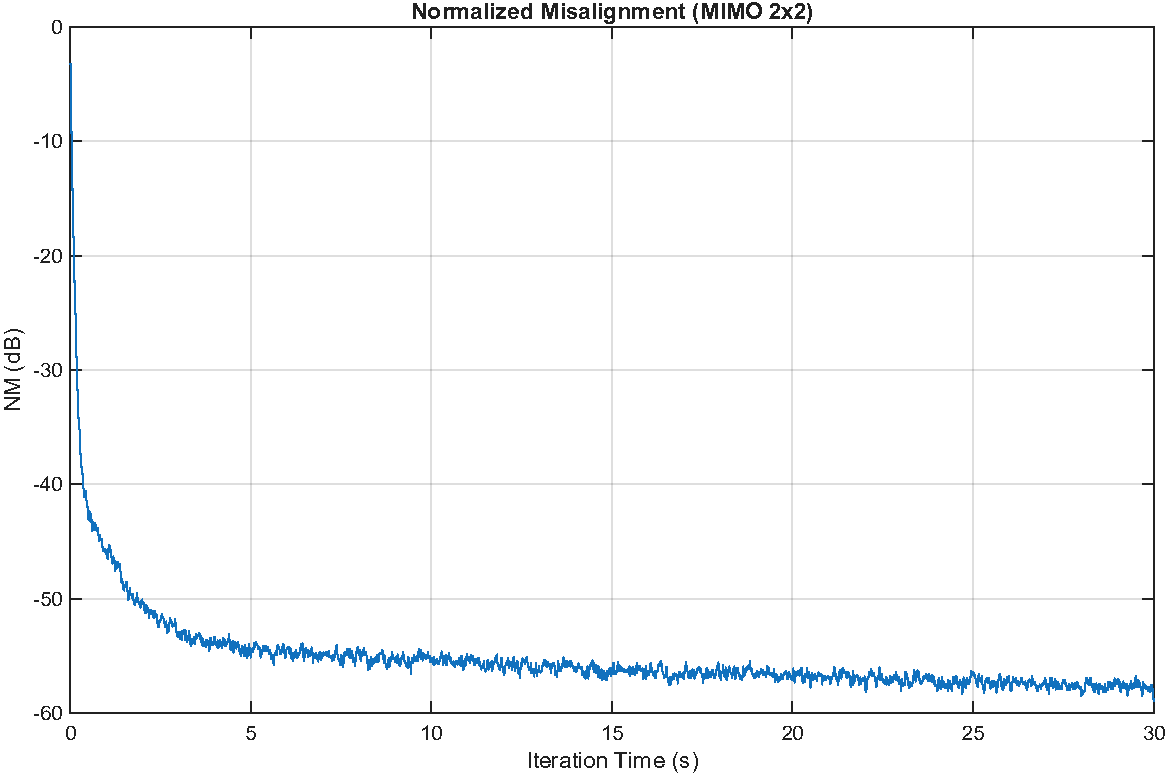
\includegraphics[width=0.8\textwidth]{plots/nm_mimo_ideal}
		\caption{\ac{nm} nel caso \ac{mimo} con ingressi scorrelati (caso ideale). Frequenza di campionamento $f_s=\SI{16}{\kilo\hertz}$.}
		\label{fig:nm_mimo_ind}
	\end{figure}
	
	Rispetto al caso \ac{siso}, l'estensione \ac{mimo} introduce alcune differenze nell'algoritmo.
	Il sistema non stima più una singola RIR, ma l'intera matrice di risposte tra ogni coppia altoparlante-microfono.
	In ciascuna sottobanda, il filtro adattativo diventa quindi una matrice $\mathbf{\hat{H}}_i$ di dimensione $M\times(L\cdot K_i)$, e l'errore di stima è calcolato simultaneamente su M microfoni.
	
	Come atteso, la stima ottenuta è praticamente perfetta: la \ac{rir} ricostruita (Figura \ref{fig:rir_mimo}) si sovrappone a quella reale sia nel dominio del tempo sia in quello della frequenza, senza scostamenti apprezzabili.
	Il test conferma quindi quanto anticipato: in assenza del problema di identificabilità, la struttura dell'algoritmo \ac{mimo} di tracciamento è corretta e ricostruisce fedelmente le risposte impulsive.
	
	\begin{figure}[H]
		\centering
		\begin{subfigure}{0.49\textwidth}
			\centering
			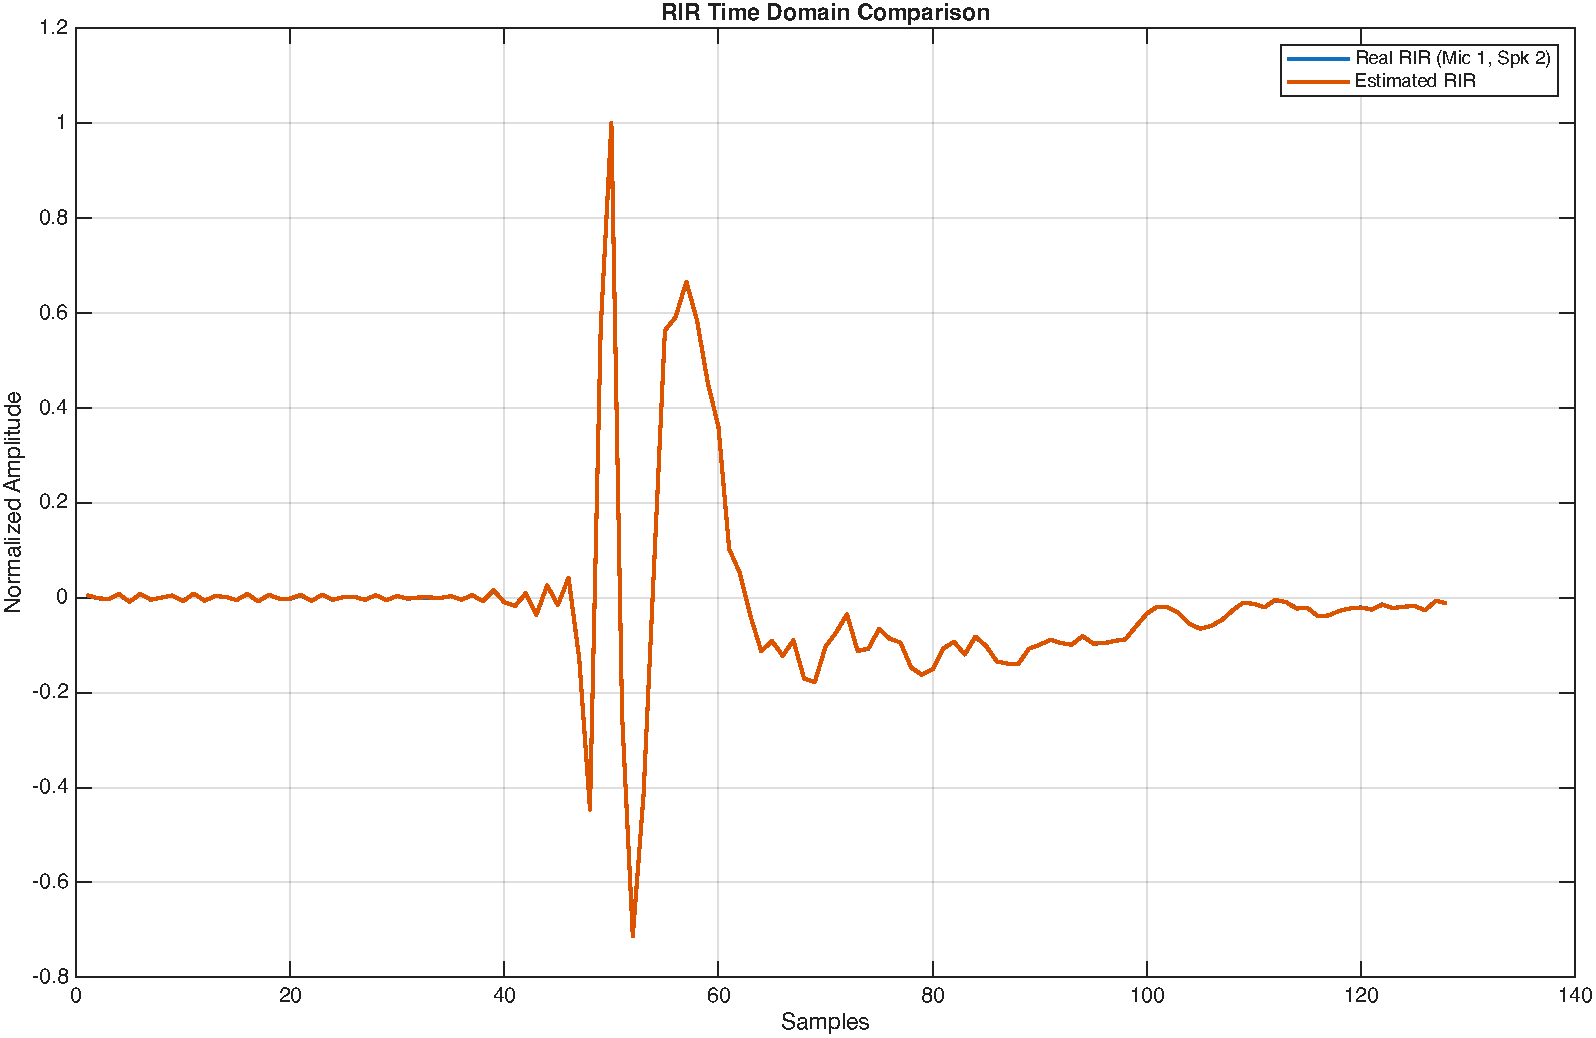
\includegraphics[width=\textwidth]{plots/rir_time_decorr}
		\end{subfigure}
		\hfill
		\begin{subfigure}{0.49\textwidth}
			\centering
			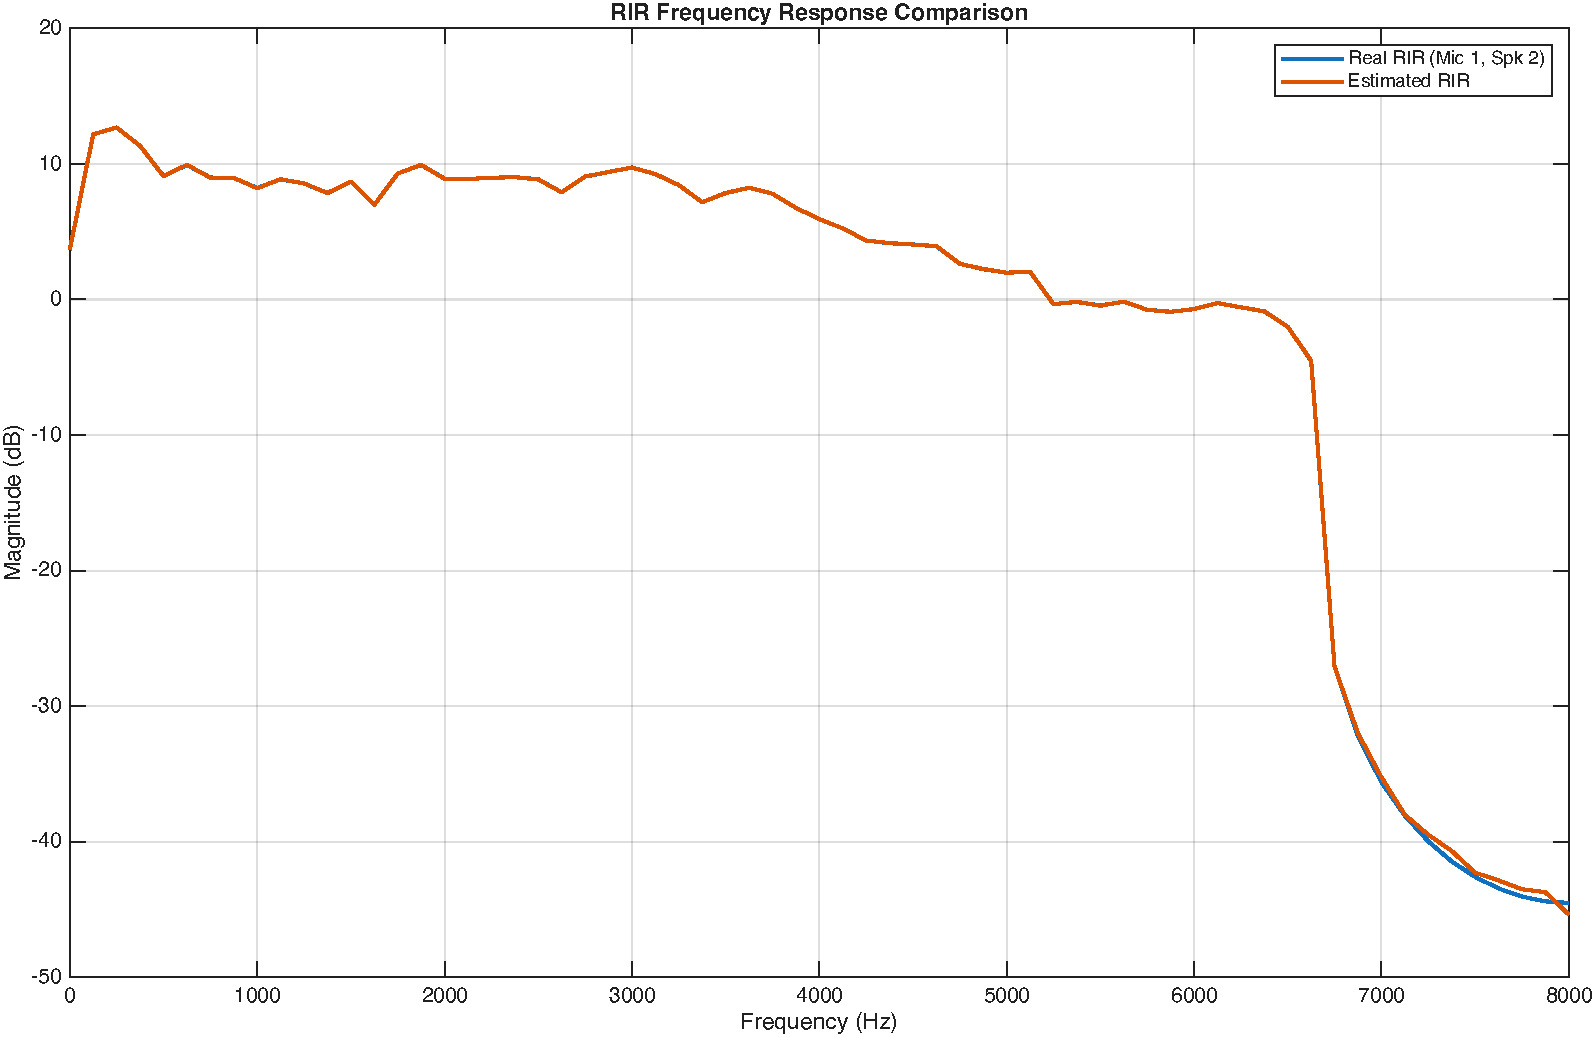
\includegraphics[width=\textwidth]{plots/rir_spectrum_decorr}
		\end{subfigure}
		\caption{\ac{rir} stimata nel caso \ac{mimo} con ingressi scorrelati, confrontata con quella reale: dominio del tempo a sinistra e dominio della frequenza a destra.}
		\label{fig:rir_mimo}
	\end{figure}
	
	\subsubsection{Ruolo della decorrelazione intra-canale ($P$)}
	Oltre alla decorrelazione tra canali (modulazione di fase), l'algoritmo IMSAF prevede una decorrelazione \emph{intra-canale} basata su una predizione lineare di ordine $P$, che sbianca il segnale di ingresso di ciascun canale.
	Con eccitazione a rumore bianco l'effetto di tale stadio non è rilevabile, poiché il segnale è già spettralmente piatto.
	Per evidenziarne il ruolo si è quindi utilizzato come ingresso un rumore colorato, applicando un filtro passabasso all'eccitazione a spettro piatto per ottenere rumore marrone.
	
	I risultati (Figura \ref{fig:nm_p_comparison}) mostrano che la decorrelazione intra-canale \textbf{accelera la velocità di convergenza senza modificare il floor} del NM. 
	A titolo di esempio, nel caso a canali scorrelati il NM raggiunge \SI{-50}{\decibel} dopo circa 150 secondi con $P=0$ e dopo soli 20 secondi con $P=2$ (circa $7.5$ volte più veloce), con floor finali paragonabili.
	Questo conferma quanto riportato in letteratura \cite{11464373}: lo sbiancamento dell'ingresso migliora la velocità di adattamento ma non il livello di errore a regime, che dipende da altri fattori (tra cui aliasing del banco, identificabilità).
	
	\begin{figure}[H]
		\centering
		\begin{tikzpicture}
			\begin{axis}[
				title={Normalized Misalignment Comparison},
				title style={font=\sffamily\bfseries\small},
				xlabel={Iteration Time (s)},
				ylabel={NM (dB)},
				label style={font=\sffamily\small},
				tick label style={font=\sffamily\footnotesize},
				legend style={font=\sffamily\small},
				xmin=0,
				x tick label style={/pgf/number format/1000 sep={}},
				grid=both,
				grid style={gray!20},
				width=0.9\textwidth,
				height=0.55\textwidth,
				legend pos=north east,
				legend cell align=left,
				tick align=inside,
				no markers,
				font=\sffamily
				]
				\addplot[black, line width=0.8pt] table [x index=0, y index=1] {plots/nm_decorr_P0_d20.dat};
				\addlegendentry{P=0}
				\addplot[matlabblue, line width=0.8pt] table [x index=0, y index=1] {plots/nm_decorr_P2_d20.dat};
				\addlegendentry{P=2}
			\end{axis}
		\end{tikzpicture}
		\caption{Confronto nel dominio della frequenza tra la RIR reale e le RIR stimate con i due prototipi.}
		\label{fig:nm_p_comparison}
	\end{figure}
	
	\subsubsection{Segnali reali e gestione pratica}\label{ssec:real_signals}
	Il passaggio da segnali sintetici a segnali audio reali introduce alcune problematiche pratiche, affrontate con due accorgimenti.
	In primo luogo, la regolarizzazione nel calcolo dei pesi sottobanda è stata resa proporzionale all'energia massima delle sottobande, anziché fissa, per garantire robustezza al variare del segnale.
	In secondo luogo, i campioni a energia molto bassa (silenzi, frequenti nei segnali reali) vengono saltati nell'aggiornamento del filtro, poichè la normalizzazione su ingresso quasi nullo porterebbe l'algoritmo a divergere.
	
	Si è inoltre confrontato l'uso di un canale mono replicato su tutti i canali con quello di un segnale stereo inviato a canali distinti.
	Il caso stereo fornisce prestazioni migliori poiché i canali sono già intrinsecamente diversi all'origine e parte del problema di identificabilità risulta attenuato a monte.
	Il segnale stereo reale rappresenta quindi un caso intermedio tra mono replicato (canali identici, caso peggiore) e ingressi indipendenti (caso ideale).

	Entrambi i segnali sono stati reperiti dal database pubblicato in \cite{ebu_sqam_flac}. Nello specifico, come segnale mono si è scelta la traccia \texttt{50.flac} (Male speech, English), e come segnale stereo la traccia \texttt{69.flac} (ABBA). I segnali, originariamente campionati a \SI{44.1}{\kilo\hertz}, sono stati ricampionati a \SI{16}{\kilo\hertz}: da un lato ciò allinea il setup a quello adottato in \cite{11464373}; dall'altro concentra l'analisi nella banda in cui il contenuto informativo del segnale e della \ac{rir} è effettivamente presente, evitando di ripartire le sottobande su una regione ad alta frequenza scarsamente eccitata. In entrambi i casi si sono impostati i seguenti parametri:
	\begin{itemize}
		\item $I = 8$, $D = 2$;
		\item $L = 2$, $M = 2$;
		\item $P = 2$;
		\item $\mu_h = 0.32$, $\delta_h = 0.001$;
	\end{itemize}
	e come filtro prototipo un coseno rialzato con $\beta = 0.6$ e \texttt{span} pari a $16$, per un totale di $129$ campioni.

	Come si nota dalle Figure \ref{fig:nm_mono_real}, \ref{fig:rir_spec_mono}, il fatto che i due canali trasmettano esattamente lo stesso segnale limita fortemente le prestazioni dell'algoritmo, introducendo una distorsione considerevole della RIR alle basse e alle alte frequenze.

	\begin{figure}[H]
		\centering
		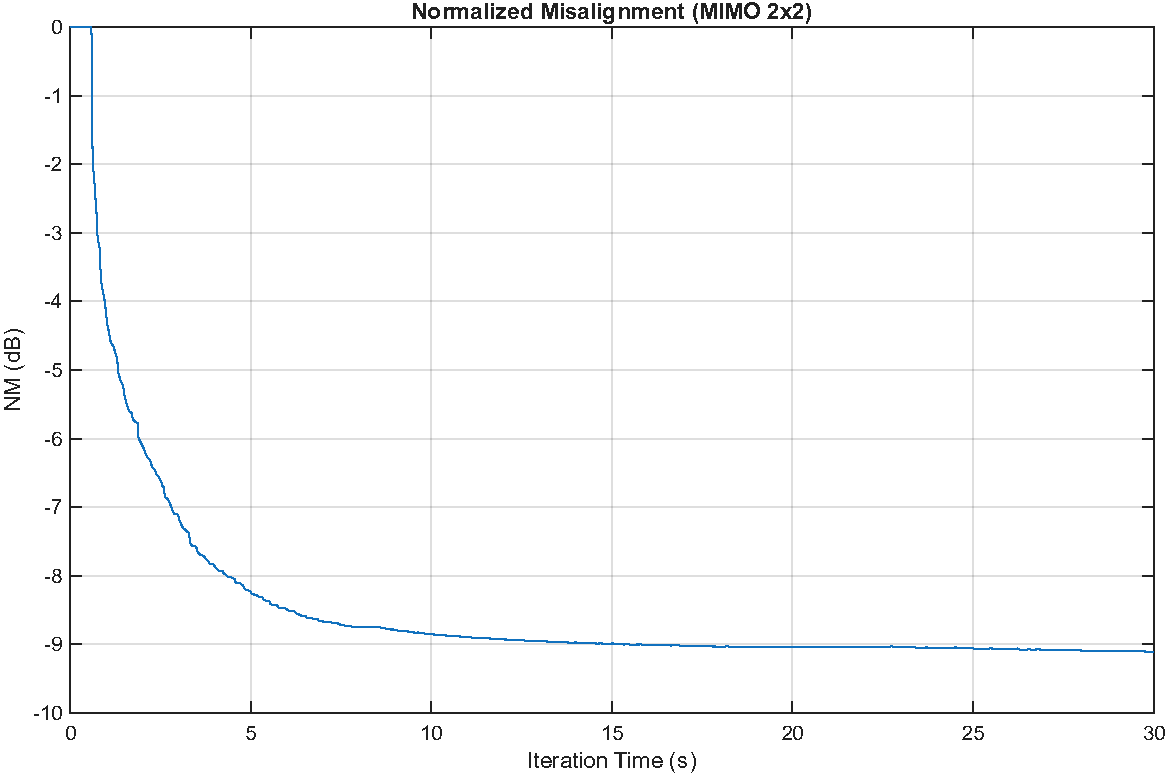
\includegraphics[width=0.8\textwidth]{plots/nm_mono_real.pdf}
		\caption{NM nel caso MIMO con ingresso mono replicato sui canali.}
		\label{fig:nm_mono_real}
	\end{figure}

	\begin{figure}[H]
		\centering
		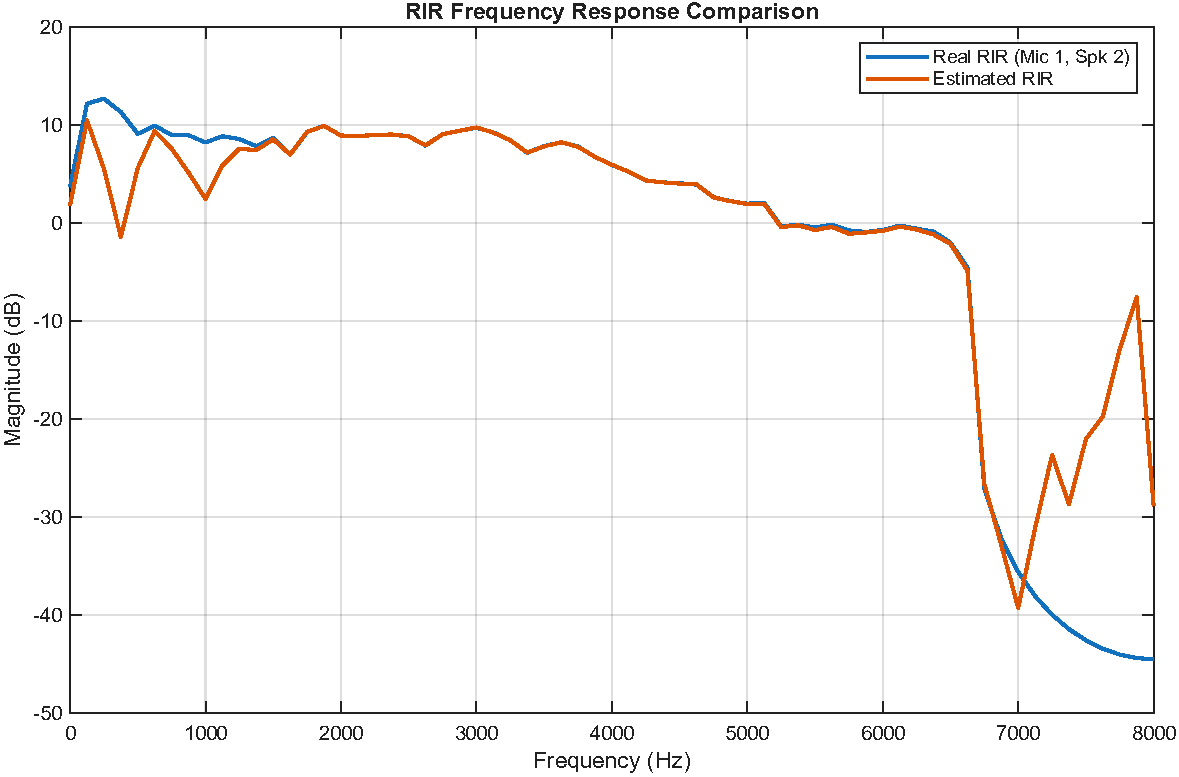
\includegraphics[width=0.8\textwidth]{plots/rir_spectrum_mono.pdf}
		\caption{Modulo della trasformata della RIR reale (blu) e stimata (arancio) con ingresso mono replicato sui canali.}
		\label{fig:rir_spec_mono}
	\end{figure}

	Al contrario, le Figure \ref{fig:nm_stereo_real}, \ref{fig:rir_spec_stereo} evidenziano che, quando i segnali trasmessi sui canali sono diversi (seppur leggermente, come avviene nel caso di due componenti di un segnale stereo), le operazioni di decorrelazione hanno un risultato migliore e portano a tracciamenti molto più accurati.
	In questo caso, infatti, il confronto tra le Figure \ref{fig:nm_mono_real} e \ref{fig:nm_stereo_real} mostra che con segnali diversificati il NM scende regolarmente allo scorrere dei campioni. 
	Inoltre, dalle Figure \ref{fig:rir_spec_mono} e \ref{fig:rir_spec_stereo} si evince che il contenuto spettrale della \ac{rir} ricostruita con segnali stereo risulta essere molto più vicino a quello della \ac{rir} reale, introducendo un significativo miglioramento nel tracciamento delle basse frequenze. 
	Anche il tracciamento delle alte frequenze migliora notevolmente ma continua a soffrire il fatto che i segnali di ingresso, in quanto segnali audio reali, sono tipicamente passa-basso e, per tale ragione, le loro sottobande relative alle frequenze più alte hanno energie molto basse.
	\begin{figure}[H]
		\centering
		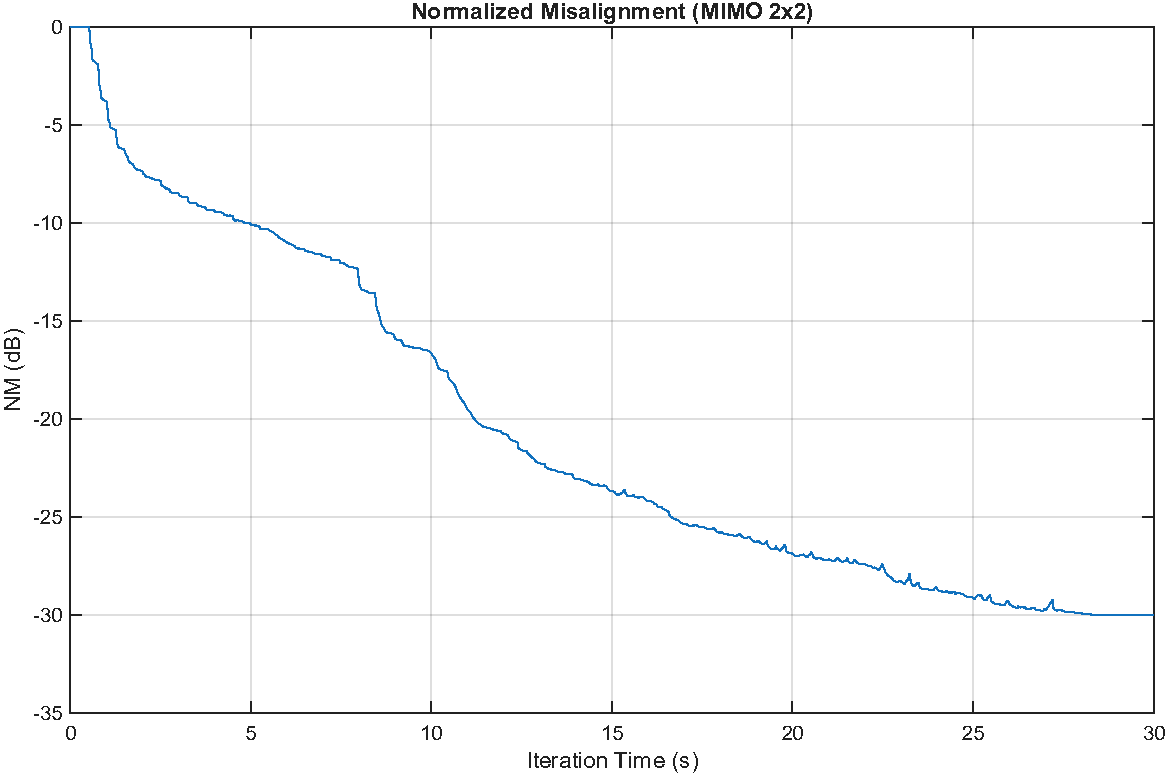
\includegraphics[width=0.8\textwidth]{plots/nm_stereo_real.pdf}
		\caption{NM nel caso MIMO con ingresso stereo diversificato sui canali.}
		\label{fig:nm_stereo_real}
	\end{figure}

	\begin{figure}[H]
		\centering
		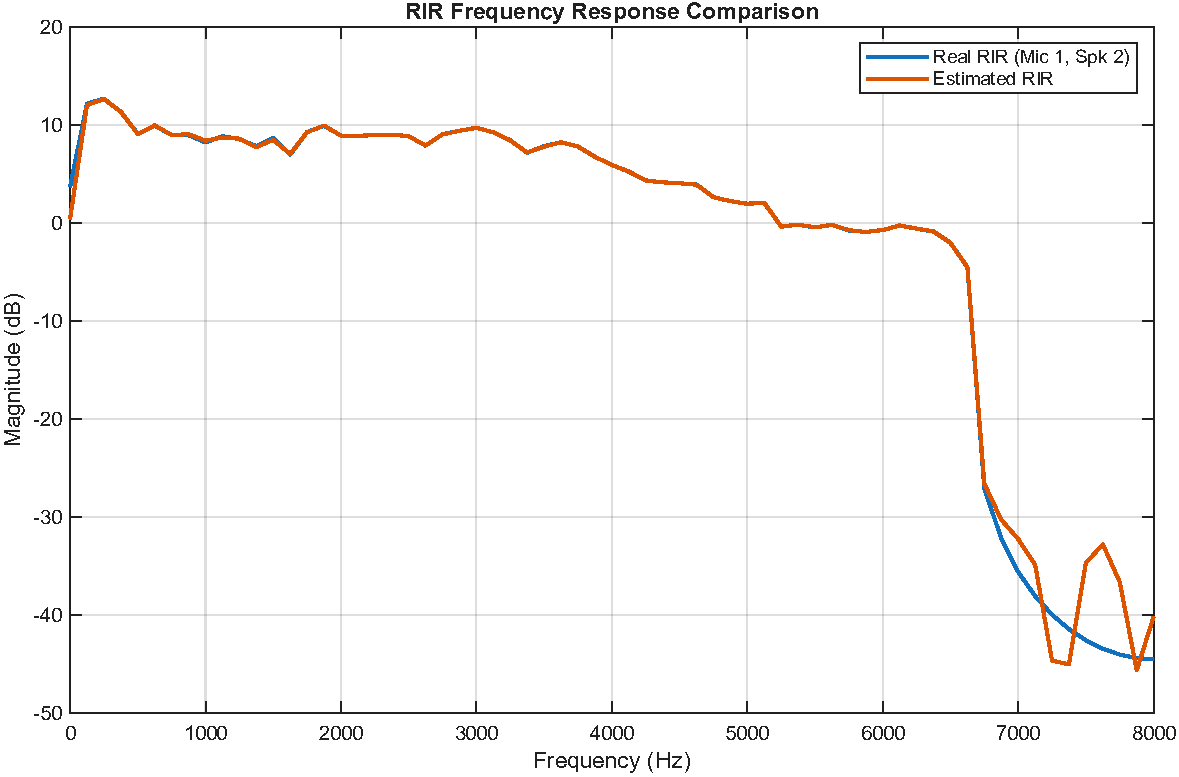
\includegraphics[width=0.8\textwidth]{plots/rir_spectrum_stereo.pdf}
		\caption{Modulo della trasformata della RIR reale (blu) e stimata (arancio) con ingresso stereo diversificato sui canali.}
		\label{fig:rir_spec_stereo}
	\end{figure}
	
	\subsubsection{Effetto del numero di sottobande}\label{ssec:subband_sweep}
	Per completezza si sono analizzate le prestazioni al variare del numero di sottobande $I$, con fattore di decimazione $D = I/4$ (per $I \geq 8$), riprendendo il setup della Sez. \ref{ssec:real_signals}: segnale stereo (\texttt{69.flac}), configurazione $2 \times 2$ e i medesimi parametri, con l'unica variazione di $I$, $D$ e $\delta_h$ posto pari a $0.01$. Sono state confrontate le configurazioni $I = 1, 4, 8, 16, 32, 64$; il caso $I = 1$, $D = 1$ corrisponde all'\ac{nlms} classico a banda piena e funge da riferimento senza decomposizione in sottobande.
	
	La Figura~\ref{fig:nm_subband_sweep} mostra un comportamento non monotono: le prestazioni migliorano all'aumentare di $I$ fino a un ottimo, per poi degradare. Il riferimento \ac{nlms} ($I = 1$) si arresta attorno a $-12$~\si{\decibel}, superato da tutte le configurazioni in sottobande a eccezione di $I = 64$: ciò conferma il vantaggio dell'approccio a sottobande, che decorrela l'ingresso e ne accelera la convergenza. L'ottimo si ha per $I = 8$ ($D = 2$), che raggiunge il floor più basso (circa $-30$~\si{\decibel}) con la convergenza più rapida; oltre tale valore la tendenza si inverte e le prestazioni degradano progressivamente, fino a $I = 64$ che scende appena sotto il riferimento fullband.
	
	Il degrado alle alte $I$ è legato all'eccitazione delle sottobande. Suddividendo un segnale reale, tipicamente passa-basso, in un numero crescente di sottobande, ciascuna sottobanda diventa più stretta e riceve una porzione di energia inferiore: le sottobande relative alle alte frequenze risultano scarsamente eccitate e vengono stimate con difficoltà. Inoltre, con $D = I/4$ la decimazione cresce con $I$, riducendo il numero di campioni disponibili per sottobanda e rallentando la convergenza.
	
	Per il segnale e la durata considerati, $I = 8$ rappresenta quindi il miglior compromesso: un numero di sottobande sufficiente a decorrelare l'ingresso, senza frammentare eccessivamente lo spettro in sottobande sotto-eccitate.
	\begin{figure}[H]
		\centering
		\begin{tikzpicture}
			\begin{axis}[
				title={Normalized Misalignment Comparison (MIMO 2x2)},
				title style={font=\sffamily\bfseries\small},
				xlabel={Iteration Time (s)},
				ylabel={NM (dB)},
				label style={font=\sffamily\small},
				tick label style={font=\sffamily\footnotesize},
				legend style={font=\sffamily\small},
				xmin=0, xmax=30.25,
				ymax=0, ymin=-30.5,
				ytick distance=5,
				grid=both,
				grid style={gray!20},
				width=0.9\textwidth,
				height=0.525\textwidth,
				legend pos=south west,
				legend cell align=left,
				tick align=inside,      
				no markers,
				font=\sffamily,
				every axis plot/.append style={line width=1pt}
				]
				\addplot[matlabblue]   table {plots/nm_i1_d1.dat};
				\addlegendentry{I=1, D=1}
				\addplot[red]   table {plots/nm_i4_d2.dat};
				\addlegendentry{I=4, D=2}%{I=4, D=1} non converge
				\addplot[magenta]   table {plots/nm_i8_d2.dat};
				\addlegendentry{I=8, D=2}
				\addplot[matlaborange]   table {plots/nm_i16_d4.dat};
				\addlegendentry{I=16, D=4}
				\addplot[violet] table {plots/nm_i32_d8.dat};
				\addlegendentry{I=32, D=8}
				\addplot[teal]   table {plots/nm_i64_d16.dat};
				\addlegendentry{I=64, D=16}
			\end{axis}
		\end{tikzpicture}
		\caption{\ac{nm} al variare del numero di sottobande $I$.}
		\label{fig:nm_subband_sweep}
	\end{figure}
	
	La Figura \ref{fig:rir_spectrum_subband_sweep} riporta il confronto tra la risposta in frequenza reale e le stime al variare di $I$.
	Le stime a sottobande seguono la risposta reale nella banda in cui questa ha contenuto : $I = 8$ vi aderisce in maniera praticamente perfetta su tutta la banda, mentre $I = 64$ inizia a discostarsi dalle medie frequenze (oltre circa \SI{4.5}{\kilo\hertz}). Il degrado di $I = 64$ è coerente con il floor più elevato mostrato dal \ac{nm} (Fig.~\ref{fig:nm_subband_sweep}) e con la scarsa eccitazione delle sottobande alte.
	Il caso \ac{nlms} a banda piena ($I = 1$) mostra invece uno scostamento sistematico, in particolare una sottostima del modulo alle basse-medie frequenze e una sovrastima alle alte: senza la decomposizione in sottobande l'adattamento converge più lentamente e non raggiunge la stessa accuratezza spettrale.
	
	\begin{figure}[H]
		\centering
		\begin{tikzpicture}
			\begin{axis}[
				title={RIR Frequency Response Comparison},
				title style={font=\sffamily\bfseries\small},
				xlabel={Frequency (Hz)},
				ylabel={Magnitude (dB)},
				label style={font=\sffamily\small},
				tick label style={font=\sffamily\footnotesize},
				legend style={font=\sffamily\small},
				x tick label style={/pgf/number format/1000 sep={}},
				xmin=0, xmax=8000,
				grid=both,
				grid style={gray!20},
				width=0.9\textwidth,
				height=0.525\textwidth,
				legend pos=south west,
				legend cell align=left,
				tick align=inside,
				no markers,
				font=\sffamily
				]
				\addplot[black, line width=1.5pt] table {plots/rir_spectrum_real.dat};
				\addlegendentry{Real RIR}
				\addplot[matlabblue, line width=0.6pt]   table {plots/rir_spectrum_i1_d1.dat};
				\addlegendentry{I=1, D=1}
				\addplot[magenta, line width=0.6pt]   table {plots/rir_spectrum_i8_d2.dat};
				\addlegendentry{I=8, D=2}
				\addplot[teal, line width=0.6pt]   table {plots/rir_spectrum_i64_d16.dat};
				\addlegendentry{I=64, D=16}
			\end{axis}
		\end{tikzpicture}
		\caption{Confronto nel dominio della frequenza tra la \ac{rir} reale e quelle stimate al variare di $I$.}
		\label{fig:rir_spectrum_subband_sweep}
	\end{figure}
	
	\subsubsection{Effetto del numero di altoparlanti}\label{ssec:l_sweep}
	È la molteplicità delle sorgenti a determinare la difficoltà di identificazione: più altoparlanti significano più \ac{rir} indipendenti da separare a partire dalle stesse osservazioni. 
	Si sono quindi analizzate le prestazioni all'aumentare del numero di altoparlanti $L$, mantenendo fisso il numero di microfoni a $M = 2$. 
	Come segnale multicanale si è impiegata la traccia \texttt{hornWag.flac} del dataset \cite{ebu_tech3324} (traccia $5.1$, di cui si è scartato il canale \ac{lfe} a bassa frequenza, utilizzando i cinque canali a banda piena FL, FR, FC, SL, SR); i canali sono stati assegnati agli altoparlanti in ordine, aggiungendone uno alla volta. 
	Sono stati adottati i medesimi parametri della Sez. \ref{ssec:subband_sweep}, con il numero di sottobande fissato al valore ottimo $I = 8$ ($D = 2$). 
	
	La Figura \ref{fig:nm_l_sweep} mostra un degrado marcato all'aumentare di $L$: il floor del \ac{nm} passa da circa $-40$~\si{\decibel} per $L = 2$ a circa $-28$~\si{\decibel} per $L = 5$, peggiorando in modo progressivo. 
	Il motivo è che ogni microfono registra la somma dei contributi di tutti gli altoparlanti: più sorgenti attive significano più contributi sovrapposti nella stessa registrazione, che l'algoritmo deve separare per stimare le singole \ac{rir}. 
	Il compito è tanto più arduo quanto più i segnali agli altoparlanti si somigliano tra loro; e sebbene un contenuto multicanale spaziale non sia una semplice copia dei canali su ogni altoparlante, i segnali restano comunque parzialmente correlati, poiché derivano dalla stessa scena sonora. 
	Aumentando $L$ cresce dunque il numero di contributi correlati da distinguere all'interno della stessa somma, e la stima peggiora.
	
	\begin{figure}[H]
		\centering
		\begin{tikzpicture}
			\begin{axis}[
				title={Normalized Misalignment Comparison (MIMO 2xL)},
				title style={font=\sffamily\bfseries\small},
				xlabel={Iteration Time (s)},
				ylabel={NM (dB)},
				label style={font=\sffamily\small},
				tick label style={font=\sffamily\footnotesize},
				legend style={font=\sffamily\small},
				xmin=0, xmax=30.25,
				ymax=0, ymin=-43,
				ytick distance=5,
				grid=both,
				grid style={gray!20},
				width=0.9\textwidth,
				height=0.525\textwidth,
				legend pos=south west,
				legend cell align=left,
				tick align=inside,      
				no markers,
				font=\sffamily,
				every axis plot/.append style={line width=1pt}
				]
				\addplot[matlabblue]   table {plots/nm_mimo_2x2.dat};
				\addlegendentry{L=2}
				\addplot[red]   table {plots/nm_mimo_2x3.dat};
				\addlegendentry{L=3}
				\addplot[magenta]   table {plots/nm_mimo_2x4.dat};
				\addlegendentry{L=4}
				\addplot[matlaborange]   table {plots/nm_mimo_2x5.dat};
				\addlegendentry{L=5}
			\end{axis}
		\end{tikzpicture}
		\caption{\ac{nm} all'aumentare del numero di altoparlanti $L$ ($M = 2$ fisso).}
		\label{fig:nm_l_sweep}
	\end{figure}
	
	\subsubsection{Effetto del numero di microfoni}\label{ssec:m_sweep}
	Per contrasto, si è fatto variare il numero di microfoni $M$ mantenendo fisso il numero di altoparlanti a $L = 2$, con lo stesso segnale e gli stessi parametri della Sez. \ref{ssec:l_sweep}.
	
	La Figura \ref{fig:nm_m_sweep} mostra che il numero di microfoni ha un effetto trascurabile: le configurazioni $M = 3, 4, 5$ sono praticamente sovrapposte tra loro e si assestano circa \SI{3}{\decibel} \emph{sopra} il caso $M = 2$, ovvero a un floor lievemente peggiore. 
	A differenza di quanto avviene per $L$, aumentare $M$ non modifica sostanzialmente le prestazioni.
	
	La ragione è che aggiungere microfoni fornisce ulteriori osservazioni dello stesso problema, ma non ne riduce la difficoltà: la separabilità degli altoparlanti dipende dalla correlazione tra i segnali di eccitazione, non dal numero di punti di osservazione. 
	Il numero di sorgenti da separare resta infatti fissato da $L$, indipendentemente da quanti microfoni ascoltano.
	
	\begin{figure}[H]
		\centering
		\begin{tikzpicture}
			\begin{axis}[
				title={Normalized Misalignment Comparison (MIMO Mx2)},
				title style={font=\sffamily\bfseries\small},
				xlabel={Iteration Time (s)},
				ylabel={NM (dB)},
				label style={font=\sffamily\small},
				tick label style={font=\sffamily\footnotesize},
				legend style={font=\sffamily\small},
				xmin=0, xmax=30.25,
				ymax=0, ymin=-43,
				ytick distance=5,
				grid=both,
				grid style={gray!20},
				width=0.9\textwidth,
				height=0.525\textwidth,
				legend pos=south west,
				legend cell align=left,
				tick align=inside,      
				no markers,
				font=\sffamily,
				every axis plot/.append style={line width=1pt}
				]
				\addplot[matlabblue]   table {plots/nm_mimo_2x2.dat};
				\addlegendentry{M=2}
				\addplot[red]   table {plots/nm_mimo_3x2.dat};
				\addlegendentry{M=3}
				\addplot[magenta]   table {plots/nm_mimo_4x2.dat};
				\addlegendentry{M=4}
				\addplot[matlaborange]   table {plots/nm_mimo_5x2.dat};
				\addlegendentry{M=5}
			\end{axis}
		\end{tikzpicture}
		\caption{\ac{nm} all'aumentare del numero di microfoni $M$ ($L = 2$ fisso).}
		\label{fig:nm_m_sweep}
	\end{figure}
	
	\subsubsection{Effetto della lunghezza della RIR}\label{ssec:rir_length}
	L'ultimo aspetto analizzato è la lunghezza $K$ della \ac{rir} stimata. 
	Finora si è adottato $K = 128$, valore ripreso da \cite{11464373}; a \SI{16}{\kilo\hertz} esso corrisponde però a soli \SI{8}{\milli\second}, sufficienti a rappresentare il suono diretto e i primi riflessi ma non la coda riverberante di un ambiente reale, il cui tempo di riverbero è tipicamente dell'ordine delle centinaia di \si{\milli\second}.
	Per valutarne l'effetto si è fatta variare $K$ da $128$ a $4096$ campioni (da \SI{8}{\milli\second} a \SI{256}{\milli\second}), mantenendo invariati gli altri parametri e la configurazione ottima delle sezioni precedenti ($I = 8$, $D = 2$, $2 \times 2$, segnale stereo ricavato da FR e FL di \texttt{hornWag.flac}).
	
	Per ciascun valore di $K$ si sono misurati il floor del \ac{nm} a regime, l'accuratezza raggiunta dopo \SI{15}{\second} di adattamento e il tempo di esecuzione, quest'ultimo normalizzato rispetto al caso base $K = 128$ per evidenziare il costo relativo indipendentemente dalla macchina.
	I risultati sono riportati in Tabella \ref{tab:rir_length}.
	
	\begin{table}[H]
		\centering
		\begin{tabular}{ccccc}
			\hline
			$K$ (tap) & Durata (\si{\milli\second}) & Floor \ac{nm} (\si{\decibel}) & $t_{exec}$ norm. & \ac{nm} a \SI{15}{\second} (\si{\decibel}) \\
			\hline
			128  & 8.0   & $-40.5$ & 1.00 & $-34.7$ \\
			256  & 16.0  & $-34.1$ & 1.31 & $-26.6$ \\
			512  & 32.0  & $-29.8$ & 1.78 & $-21.7$ \\
			1024 & 64.0  & $-21.3$ & 2.80 & $-16.7$ \\
			2048 & 128.0 & $-16.7$ & 6.29 & $-13.2$ \\
			4096 & 256.0 & $-13.0$ & 9.26 & $-10.3$ \\
			\hline
		\end{tabular}
		\caption{Effetto della lunghezza $K$ della \ac{rir} sul floor del \ac{nm}, sull'accuratezza a \SI{15}{\second} e sul tempo di esecuzione (normalizzato al caso $K = 128$). Configurazione $I = 8$, $D = 2$, $2 \times 2$, $f_s = \SI{16}{\kilo\hertz}$.}
		\label{tab:rir_length}
	\end{table}
	
	La tabella evidenzia un compromesso netto. 
	All'aumentare di $K$ il floor del \ac{nm} peggiora in modo monotono, da $-40.5$ \si{\decibel} per $K = 128$ fino a $- 13.0$ \si{\decibel} per $K = 4096$: stimare un numero crescente di coefficienti a parità di eccitazione rende il problema più difficile e la stima meno accurata a regime.
	Parallelamente il costo computazionale cresce fino a oltre nove volte quello del caso base.
	Il degrado si concentra inoltre alle alte frequenze, dove la coda riverberante che si aggiunge allungando la \ac{rir} è meno eccitata dal segnale, tipicamente passa-basso.
	
	Si evidenzia quindi la natura di compromesso della scelta di $K$: valori piccoli, come i \SI{8}{\milli\second} adottati in letteratura, garantiscono floor e convergenza migliori ma descrivono la stanza in modo incompleto, trascurando la coda riverberante; valori maggiori catturano una porzione più realistica della \ac{rir}, al prezzo di un floor più elevato e di un tempo di calcolo sensibilmente maggiore.
	
	\section{Implementazione C++}
	
	\newpage
	\bibliographystyle{ieeetr}
	\bibliography{references/refs}
\end{document}
